\documentclass[fontsize=12pt, paper=a4, headinclude, twoside=false, parskip=half+, pagesize=auto, numbers=noenddot, open=right, toc=listof, toc=bibliography]{scrreprt}

%\usepackage[inner=4cm,outer=2cm]{geometry}
%\setlength{\oddsidemargin}{15,5pt}
%\setlength{\evensidemargin}{15,5pt}


%parskip:
  % full - Absätze haben großen Abstand
  % half - Absätze haben kleinen Abstand
  % off - Absätze haben Einzug (default)

% Bessere Unterstützung für PDF-Features
\usepackage[breaklinks=true]{hyperref}

%Schönere Schriftart laden
%\usepackage[latin1]{inputenc}
\usepackage[T1]{fontenc} % Ligaturen, richtige Umlaute im PDF
\usepackage[utf8]{inputenc}% UTF8-Kodierung für Umlaute usw
\usepackage[english]{babel} % Deutsche Silbentrennung verwenden
\usepackage{lmodern}
\renewcommand*\familydefault{\sfdefault}  %Zusatz für serifenlose Schrift.

%Zeilenabstand
\usepackage{setspace} % Zeilenabstand
\onehalfspacing % 1,5 Zeilen

% Schriften-Größen
\setkomafont{chapter}{\Huge\rmfamily} % Überschrift der Ebene
\setkomafont{section}{\Large\rmfamily}
\setkomafont{subsection}{\large\rmfamily}
\setkomafont{subsubsection}{\large\rmfamily}
\setkomafont{chapterentry}{\large\rmfamily} % Überschrift der Ebene in Inhaltsverzeichnis
\setkomafont{descriptionlabel}{\bfseries\rmfamily} % für description Umgebungen
\setkomafont{captionlabel}{\small\bfseries}
\setkomafont{caption}{\small}



% Einfachere Verwendung von korrekten Anführungszeichen
\usepackage[german=guillemets]{csquotes}
% oder german=quotes
% oder english=british oder english=american

%Mathematisches
\usepackage{amssymb}
\usepackage{amsmath}
\usepackage{amsthm}

%Quelltext einbinden
\usepackage{algorithm}
\usepackage{algorithmic}

%Abbildungen
\usepackage{graphicx}
\usepackage{caption}
\usepackage{subcaption}
\usepackage[verbose]{wrapfig}
\usepackage{float}
%\restylefloat{figure} %kannst du einen weiteren Positionierungsparameter [H] definieren. der setzt dir das bild an genau die stelle, wo du es haben willst. Ist allerdings auch nicht immer so praktisch.
% wenn du ein \pagebreak einfügst, gibt er dir vor der neuen seite noch alle gleitobjekte aus, die noch anstehen

%Zeichnen mit Tikz
\usepackage{tikz}
\usetikzlibrary{intersections,positioning,shapes.geometric,calc}

% Tabellen
\usepackage{multirow} % Tabellen-Zellen über mehrere Zeilen
\usepackage{multicol} % mehre Spalten auf eine Seite
\usepackage{tabularx} % Für Tabellen mit vorgegeben Größen
\usepackage{longtable} % Tabellen über mehrere Seiten
\usepackage{array}

%Bibliographie
\usepackage[square, comma, numbers, sort&compress, round]{natbib}
\usepackage{bibgerm} % Umlaute in BibTeX

%Umbenennung der vordefinierten definition- und example-Umgebung
\theoremstyle{definition}
\newtheorem{lecture}{Lecture}
\newtheorem{definition}{Definition}
\newtheorem{example}{Example}
\newtheorem{lemma}{Lemma}

% \newtheorem{theorem}{Satz}
% \newtheorem{constructing instructions}{Konstruktionsvorschrift}
% \newtheorem{properties}{Eigenschaften}
%\newtheorem{proposition}{Proposition}
%\newtheorem{korollar}{Corollary}
%\newtheorem{remark}{Remark}
%\newtheorem{consequences}{Consequences}
%\newtheorem{observation}{Observation}
%\newtheorem{conjecture}{Conjecture}
%\newtheorem{recall}{Recall}

\renewcommand{\labelenumi}{\roman{enumi})}

\renewcommand{\labelitemii}{$\bullet$}

\newcommand{\todo}[1]{
      {\colorbox{red}{ TODO: #1 }}
}
\newcommand{\todotext}[1]{
      {\color{red} TODO: #1} \normalfont
}

%bzgl `tocbasic` Warnung
\usepackage{scrhack}


\author{Lydia Buntrock}
\title{master thesis}
\date{Januar 2018}

\hfuzz=\maxdimen \tolerance=10000 \hbadness=10000
% \usepackage[showframe=true]{geometry}


\begin{document}
  \begin{titlepage}
    \pagestyle{empty}
  	\begin{center}
      {\Large Freie Universität Berlin} \\
    	\begin{Huge}
      	Fachbereich Mathematik und Informatik \\
      	\vspace{3mm}
    	\end{Huge}
    	\vspace{2cm}
    	\begin{Large}
        \textbf{An analysis of maximum parsimony algorithms to predict parasitism in Eukaryota} \\
        \vspace{3mm}
        using a large multifurcated phylogenetic synthesis tree \\
    	\end{Large}
      \vspace{3cm}
      \textbf{Submitted on:} \\
      3 April 2018 \\
    	\vspace{2cm}
    	Lydia Buntrock \\
      E-Mail: info@irallia.de \\
     	\vspace{3cm}
      \textbf{Supervisors:} \\
      Prof. Dr. Bernhard Y. Renard \\
      \& \\
      Prof. Dr. rer. nat. Emanuel Heitlinger \\      
  	\end{center}
    \clearpage
    \pagenumbering{Roman}
  \end{titlepage}

%---------------------------------------------------------------------------------------------------
%---------------------------------------------------------------------------------------------------
%---------------------------------------------------------------------------------------------------
%--------------------------------------------------------------------------------------------------- 
\chapter*{Abstract}

  Parasitism can be defined as an interaction between species in which one of the interaction 
    partners, the parasite, lives in or on the other, the host. The parasite draws food from its 
    host and harms it in the process. According to estimates, above 40\% of all Eukaryota are 
    parasites. Nevertheless, it is computationally difficult to obtain information whether a 
    particular taxon is a parasite making it difficult to query large sets of taxa.

  Here we test in how far it is possible to use the Open Tree of Life (OTL), a synthesis of 
    phylogenetic trees on a backbone taxonomy (resulting in unresolved nodes), to expand available 
    information via phylogenetic trait prediction. We use the Global Biotic Interactions (GloBI) 
    database to categorise 25,962 and 34,860 species as parasites and free-living, respectively and 
    predict states for over $\sim$2.3 million (97.34\%) leaf nodes without state information.

  We estimate the accuracy of our maximum parsimony based predictions using cross-validation and 
    simulation at 60-80\% overall, while strongly varying between clades. The cross-validation 
    results in an accuracy of 98.17\% which is explained by the fact that the data is not uniformly 
    distributed. We describe this variation across taxa as associated with available state and 
    topology information. We compare our results with several smaller scale studies which used 
    manual expert curation and conclude that computationally inferred state changes largely agree in 
    number and placement with those. In clades in which available state information is biased 
    (mostly towards parasites, e.g. in Nematodes) phylogenetic prediction is bound to provide 
    results contradicting conventional wisdom.

  This represents, to our knowledge, the first comprehensive computational reconstruction of the 
    emergence of parasitism in Eukaryota. We argue that such an approach is necessary to allow 
    further incorporation of parasitism as an important trait in species interaction databases and 
    in individual studies on Eukaryota e.g. in the microbiome.

%---------------------------------------------------------------------------------------------------

  % This study focuses on the ancestral state reconstruction of parasitism in the tree of life of
  %   Eukaryota. We predict unknown states of species and estimate origins and losses of parasitism. \\
  % The challenge here is the size of the tree and the little information about it. \\
  % Such a large phylogenetic tree does not completely exist and therefore we work with a synthesis 
  %   tree of OTL \cite{Hinchliff2015} which is highly multifurcated. \\
  % For the 2,535,437 leaf nodes we could not gather much data. From the GloBI database 
  %   \cite{Poelen2014} which we used, we could only collect 25,962 parasitic and 34,860 free-living 
  %   species. It follows that we have $\approx 2.4\%$ state information. \\
  % So far, especially small scale or highly manual studies have been carried out. In this scale, it 
  %   requires different data sources to be interconnected. \\
  % We performed an analysis of existing algorithms and selected a Sankoff maximum parsimony algorithm 
  %   using the R package \textit{castor} \cite{Louca2017}. \\
  % Nevertheless, the results are convincing and even though this is a purely computational approach 
  %   which did not include human experts input, results coincide with prior knowledge. Also regarding 
  %   the number of events, our estimates coincide with previous results by human experts, e.g. the 
  %   study by Weinstein and Kuris \cite{Weinstein2016}. \\

\tableofcontents
\clearpage
\pagenumbering{arabic}

%---------------------------------------------------------------------------------------------------
%---------------------------------------------------------------------------------------------------
%---------------------------------------------------------------------------------------------------
%--------------------------------------------------------------------------------------------------- 
\chapter{Introduction}
  This thesis is about the analysis of ancestral state reconstruction algorithms for non-binary 
    trees, applied to the currently largest phylogenetic synthesis tree of Open Tree of Life (OTL)
    \cite{Hinchliff2015} to predict parasitism in Eukaryota.

  For about 50 years, people have been working on ancestral state reconstruction, the inference of 
    evolution that leads to the given data. One of the first papers was written by Camin and Sokal, 
    who were working on algorithms for discrete-state data in 1965 \cite{Camin1965}. Different 
    methods have been developed and the question is which method is the most suitable for the 
    problem at hand: the ancestral state reconstruction for a huge non-binary tree with two discrete 
    states.

  Royer-Carenzi et al. distinguish two major classes of ancestral state reconstruction methods: The
    first is maximum parsimony: explain the current state with the least number of state changes 
    between the child and its ancestor. The other class they present describes the modeling of 
    character evolution as a stochastic process and uses the likelihoods to compute the possible 
    ancestral character states. This is generally done with a continuous time Markov model 
    \cite{RoyerCarenzi2013}.

  One of the major disadvantages of parsimony methods is that, in contrast to likelihood approaches, 
    they can not take divergence times (branch length) into account. Since the OTL does not include 
    development times of species, this can not be considered here. Another problem pointed out by 
    Royer-Carenzi is that parsimony approaches are either based on predefined parameters 
    (generalized parsimony) or on strong and often controversial assumptions, like irreversibility 
    of transitions (Dollo parsimony). This problem is unimportant to the present task because in the 
    analysis of the entire Eukaryota tree only generalized models are meaningful. The comparison of 
    methods gives us the maximum parsimony method as the simplest and fastest method that meets all 
    our requirements.

  Felsenstein \cite{Felsenstein2003} discusses in his book two parsimony algorithms that generalize 
    previous methods (from Camin and Sokal \cite{Camin1965}, Farris \cite{Farris1970} and others): 
    Fitch parsimony \cite{Fitch1971} and Sankoff parsimony \cite{Sankoff1975}. Therefore, these are 
    the methods used in this work. For Fitch, the algorithm has been extended from binary to 
    non-binary trees. For the Sankoff algorithm, Louca and Doebeli have presented an implementation 
    for non-binary trees published in an R package named \textit{castor} \cite{Louca2017}.

  For an ancestral reconstruction on the phylogeny of Eukaryota, we use Open Tree of Life (OTL) 
    \cite{Hinchliff2015}. Phylogeny describes the evolution of species, while the taxonomy is a 
    classification according to certain criteria in so-called taxa. OTL is a comprehensive, dynamic 
    and digitally available tree of life constructed from published phylogenetic trees along with a 
    backbone of taxonomic data. Besides this, Hinchliff et al. also offer an OpenTreeOfLife-Taxonomy 
    (OTT) with the help of which we identify the individual nodes. It follows that the biggest 
    'phylogenetic tree' is this synthesis of phylogenetic trees filled with a taxonomic trees given 
    by OTL.

  For these large phylogenetic synthesis trees, however, ancestral state reconstruction has so far 
    only been done for Bacteria and Archaea for binary traits by Goberna and Verdú \cite{Goberna2015}.
    However, this differs from Eukaryota in the sense that complex traits such as parasitism depend
    on more than one gene.

  The present tree structure of OTL is not binary but multifurcated, meaning that each node has
    multiple ($n > 2$) children or in other words its degree, number of adjacent nodes, is greater 
    than 3 \cite{Felsenstein2003}. Parsimonious in phylogeny refers to favoring the tree that needs 
    the least evolutionary change to explain the observed data. Maximum parsimony methods have been 
    developed for phylogenies, which are usually depicted as binary trees. Therefore, the selected 
    parsimony methods are not directly applicable, as they were specifically applied to much smaller 
    subtrees, where all splits are known. We will extend and test the existing maximum parsimony 
    algorithms of Fitch \cite{Fitch1971} and Sankoff \cite{Sankoff1975} for this task and estimate 
    their predictive power. 

  Note, the original Fitch algorithm has the sole purpose of minimizing the number of transitions 
    and not the reconstruction of the ancestral nodes. Felsenstein \cite{Felsenstein2003} describes 
    a simple extension for the reconstruction. In this work, the algorithm extended to 
    reconstruction is adapted to multifurcated trees, based on the critical reevaluation of this 
    extension by Cunningham et al. \cite{Cunningham1998}.

  To accomplish this task, information about the states of the current species is needed in addition 
    to the phylogenetic tree.  Most of the largest interaction databases (e. g. IWDB (Interaction 
    Web Database) \cite{IWDB2003}, Webs on the Web \cite{WOW2004}, Animal Diversity Web 
    \cite{Myers2003} and ecoweb \cite{Cohen2010}) are offline or outdated. We use the interaction 
    database Global Biotic Interactions (GloBI) \cite{Poelen2014} because it is including most of 
    the known databases and is still growing actively \cite{Poelen2014}. The data in GloBI is stored 
    as interactions e.g. species A parasitizes species B. We conclude that species A is parasitic 
    and species B free-living. From this data, we could specify $\sim$2.3 million leaf nodes 34,860 
    as free-living and 25,962 as parasitic. 

  There are many different ways to define parasitism. Since we use GloBI to classify species, we use 
    their definition of parasitism. In GloBi, Ontobee definitions are used \cite{Xiang2011}. The 
    interaction \textit{has parasite} is defined as: "An interaction relationship between two 
    organisms living together in more or less intimate association in a relationship in which 
    association is disadvantageous or destructive to one of the organisms."\footnote{
      \hyperlink{http://www.ontobee.org/ontology/RO?iri=http://purl.obolibrary.org/obo/RO_0002445}
      {ontobee.org/ontology/RO?iri=http://purl.obolibrary.org/obo/RO\_000244}; Last checked: 22.03.2018.
    }. This definition includes: ecto- and endoparasites, parasitoids, kleptoparasites and pathogens. \\


  The objectives of this work are the following points: (1) Find a suitable ancestral state 
    reconstruction method. (2) Accomplish reconstruction on the Eukaryota synthesis tree of OTL. The 
    goal of point 1 is to evaluate the possible methods based on a simulation of our data situation. 
    The Sankoff algorithm implemented by Louca et al. is the best in our comparisons. Therefore,
    point 2 consists of reconstructing the ancestral states, predicting the unknown leaf states with 
    the aid of this algorithm and perform an evaluation of the results.

%---------------------------------------------------------------------------------------------------
%---------------------------------------------------------------------------------------------------
%---------------------------------------------------------------------------------------------------
%--------------------------------------------------------------------------------------------------- 
\chapter{Aims}
  The primary objective of this thesis is the application of maximum parsimony algorithms to 
    non-binary trees and very large data sets to predict unknown leaf node states.

  We discuss different ancestral state reconstruction methods and test the most appropriate ones on 
    our data. Hereby, we want to find out how far it is possible to use the Open Tree of Life (OTL) 
    to expand available information via phylogenetic trait prediction. As a basis for known states, 
    we use the Global Biotic Interactions (GloBI) database, which categorises 34,860 and 25,962 
    species as free-living and parasites. This data is used to perform an ancestral state 
    reconstruction and predict states for over $\sim$2.3 million (97.34\%) leaf nodes without state 
    information.

  In order to generate a realistic simulation, influencing parameters are investigated. Since the 
    transitions are minimized in an ancestral state reconstruction, this is an important parameter 
    to consider. On the other hand, the completeness of our input data affects our data enormously.
    Therefore, two major types are distinguished:
  \begin{enumerate}
    \item Biological parameters (a result of the evolutionary process):
      \begin{itemize}
        \item State distributions and transition probabilities
      \end{itemize}
    \item Distribution of missing information:
      \begin{itemize}
        \item Lack of information on topology ($\rightarrow$ multifurcations)
        \item Lack of information of states of some leaf nodes
      \end{itemize}
  \end{enumerate}

%---------------------------------------------------------------------------------------------------
%---------------------------------------------------------------------------------------------------
%---------------------------------------------------------------------------------------------------
%--------------------------------------------------------------------------------------------------- 
\chapter{Methods}
  In this thesis, a maximum parsimony algorithm is applied to the Eukaryota tree to obtain an 
    ancestral state reconstruction of free-living versus parasite states. This chapter is divided 
    into the following sections: the description of the used data sources and the analysis of these 
    data as a preparation for the simulation. A description of the analyzed methods for the 
    ancestral state reconstruction and then an explanation of how they fit the problem at hand. And 
    at the end, the real data analysis with the Sankoff method. Figure \ref{fig:workflow} briefly 
    outlines these relationships. A more detailed view of the workflow can be found in the appendix 
    \ref{fig:BigWorkflow}.

  \begin{figure}[h!]
    \centering
    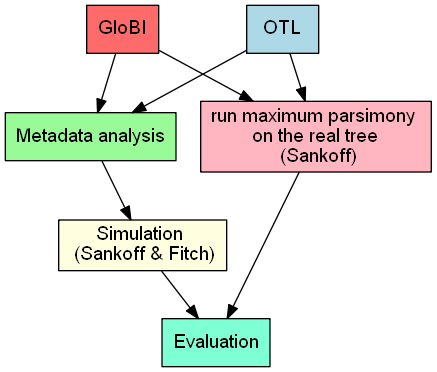
\includegraphics[width=0.49\textwidth]{Figures/Workflow-overview.png}
    \caption{The Workflow of the resulting procedure with the following steps: \\
      (1) Retrieve phylogenentic tree data as input for the tree (OTL) and the state information (GloBI).
      (2) Get metadata of these for a realistic simulation of the maximum parsimony algorithms (Fitch \& Sankoff).
      (3) Build and run the simulation.
      (4) Evaluation of parameters for the simulation and the ancestral state reconstruction of the real tree.
      (5) Evaluate the accuracy of developed algorithms and choose the best.
      (6) Run the resulting algorithm on the original data.
      (7) Evaluate and interpret the results.
    }
    \label{fig:workflow}
  \end{figure}
  
  %---------------------------------------------------------------------------------------------------
  %---------------------------------------------------------------------------------------------------
  %---------------------------------------------------------------------------------------------------
  \section{Data sources}
    Two types of data are needed for an ancestral state reconstruction: a tree and information about 
      the states.

    The database of Open Tree of Life (OTL) is used for the subsequent analysis of the Eukaryota tree
      (downloaded on 16.02.2018) \cite{Hinchliff2015}. This database gives a synthesis of phylogenetic 
      trees (currently 819 trees) and a taxonomic tree\footnote{
        \hyperlink{https://tree.opentreeoflife.org/about/synthesis-release/v9.1}
        {https://tree.opentreeoflife.org/about/synthesis-release/v9.1}; Last checked: 22.03.2018.
      }. OTL also includes the large phylogenetic database TreeBASE \cite{Hinchliff2015}.
      
    Furthermore the Open Tree Taxonomy (OTT) from OTL is used because it includes most of the known 
      taxonomies and is synthesised by preferring taxonomies that match with available phylogenetic 
      data. The team of OTL prefers a maximum number of species \cite{Hinchliff2015}, this results in 
      the synthesis between taxonomy and phylogeny.

    For the state information the Global Biotic Interactions database (GloBI) is being used
      \cite{Poelen2014} (downloaded on 29.01.2018). This database consists of interactions: species A 
      (source) interacts with B (target). A number of interactions has been 
      identified\footnote{\hyperlink{
        https://github.com/jhpoelen/eol-globi-data/blob/master/eol-globi-lib/src/main/java/org/eol/globi/domain/InteractType.java
        }{https://github.com/jhpoelen/eol-globi-data/blob/master/eol-globi-lib/src/main/java/org/eol/globi/ \\ domain/InteractType.java}; Last checked: 22.03.2018.
      }, including those indicating whether the species source or target has become a parasite or a 
      free-living species from the biological perspective. They are the following:
    \begin{itemize}
      \item free-living source: preysOn, eats, flowersVisitedBy, hasPathogen, pollinatedBy, 
        hasParasite, hostOf
      \item free-living target: preyedUponBy, parasiteOf, visitsFlowersOf, pathogenOf, hasHost
      \item parasite source: parasiteOf, pathogenOf
      \item parasite target: hasParasite, hasPathogen
    \end{itemize}

    Of these interactions (e.g. species A parasitizes species B) the state of the species is 
      determined (species A is parasitic, species B is free-living). In the case that one parasite 
      conquers another parasite (parasitizes), conflicting conditions arise for the second species.
      This is solved by preferring the parasitic state.

    For each species known identifiers are stored in GloBI. This includes OTT (the taxonomy of OTL). 
      All species that have stored an OTT identifier and have a matching interaction are divided into 
      two lists: parasites and free-livings.

  %---------------------------------------------------------------------------------------------------
  %---------------------------------------------------------------------------------------------------
  %---------------------------------------------------------------------------------------------------
  \section{Metadata analysis}
    Based on the input data, generalized linear models are compared with poisson respectively binomial 
      regression according to their residuals. In order to compare models of different complexity, the 
      BIC (Bayesian Information Criterion) values are calculated in addition to the residuals.
      
    There are two different information criteria: AIC (Akaike Information Criteria) and BIC. The 
    advantage of the BIC is that the penalty is dependent on the sample size and is therefore 
      advantageous for large samples.
      
    For all these calculations, the following R functions are  used: \textit{glm()}, \textit{anova()} 
      and \textit{BIC()}.
    % https://stat.ethz.ch/R-manual/R-devel/library/stats/html/glm.html

    For each node, depth, min, max and mean height are  noted. The node depth is calculated as the
      distance (number of edges) to the root node. The node height is calculated in three different 
      ways: min, max and mean height refers to the (mininmal, maximal, mean) distance to a leaf node.
      The influence in the modeling of these parameters is tested both additively and multiplicatively 
      on the models.

  %---------------------------------------------------------------------------------------------------
  %---------------------------------------------------------------------------------------------------
  %---------------------------------------------------------------------------------------------------
  \section{Ancestral state reconstruction methods}
    The methods used to reconstruct the ancestral states are Fitch parsimony \cite{Fitch1971} and 
      Sankoff parsimony \cite{Sankoff1975}, which are explained in the following subsections.

    %---------------------------------------------------------------------------------------------------
    %---------------------------------------------------------------------------------------------------
    \subsection{Fitch maximum parsimony}
      Based on the work of Cunningham et al. \cite{Cunningham1998} the Fitch method \cite{Fitch1971} 
        is implemented and extended by us for the multifurcated tree case. To understand the 
        differences to the multifurcated case, the algorithm for the binary case is briefly explained 
        and referred to the extension. \\
        \begin{wrapfigure}[17]{r}{0.5\textwidth}
          \centering
          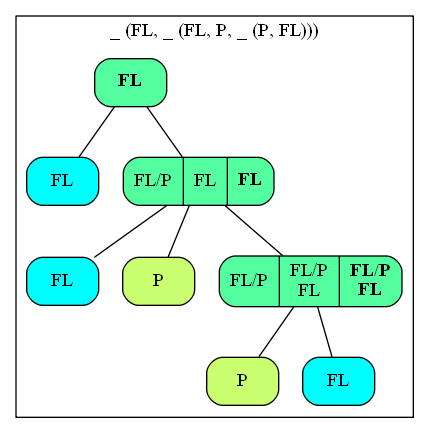
\includegraphics[width=0.4\textwidth]{Figures/Fitch1.png}
          \caption{Fitch algorithm for binary trees. \\
            The unknown leaf node is described with both states. Computed internal nodes (except for the 
            root node) consist of three sets, where the last set is the final one (bold). \\
            From the second internal node (seen from the root node) there are several possibilities to 
            create the second and third set.}
          \label{fig: binary Fitch}
        \end{wrapfigure}
      Input: A rooted binary tree with state information in the leaf nodes. Each node is depicted as 
        a set of states. There are only two states in this thesis, free-living (FL) and parasitic (P).
        Internal nodes have three sets that are empty at the beginning, except for the root node, which
        has only one. Leaf nodes have their state as a set (e.g. \{FL\} or \{P\}, unknown leaf nodes 
        have the union of all possible states (\{FL, P\}).

      The algorithm traverses three times through the tree and fills these sets. In each step, two sets 
        are considered and their intersection is formed. There are two cases:
      \begin{enumerate}
        \item The intersection is not empty and corresponds to the new set.
        \item The intersection is empty. $\rightarrow$ Build the union of these sets as new set.
      \end{enumerate}
      The first traversion goes from the leaf nodes to the root: each internal node is formed by its 
        child nodes, where the only information lies at the beginning. The Second traversion goes from 
        the root node to the leafs: each internal node is formed from its parent node and its sibling 
        node. Last traversion (direction does not matter): the final state is builded for every node. It 
        is formed from the sets of previous traversals.

      (The original Fitch algorithm is designed to minimize transitions without predicting actual states 
        of internal nodes, so it is just the first traversal.)

      The extension to the non-binary case is quite obvious, but holds some opportunities. In this case, 
        more than two children may be present for the first traversal, but the intersection or union can 
        also be formed over more than two sets. There may also be several sibling nodes in the second 
        traversing. However, there are several possibilities here that are all tested and compared in 
        the simulation. Some of these options are already available in the binary case:
      \begin{itemize}
        \item The parent node has two state sets (except for the root node), because it came through 
          the up-traversing previously. Are both sets used or only the first traversing?
        \item If there are several siblings, the cut or union could made first of these, or directly 
          including the parent node.
      \end{itemize}
      The first point already has an effect on the binary case. Figure \ref{fig: binary Fitch} shows 
        both possibilities of the three sets. Cunningham uses only the first state set of the parent 
        node \cite{Cunningham1998}. From these two points four different versions of Fitch are formed:
      \begin{enumerate}
        \item Fitch 1: First state set of parent node; intersection/union of siblings first.
        \item Fitch 2: First state set of parent node; intersection/union of siblings together with parent node.
        \item Fitch 3: Both state sets of parent node; intersection/union of siblings first.
        \item Fitch 4: Both state sets of parent node; intersection/union of siblings together with parent node sets.
      \end{enumerate}

      \begin{figure}[h!]
        \centering
        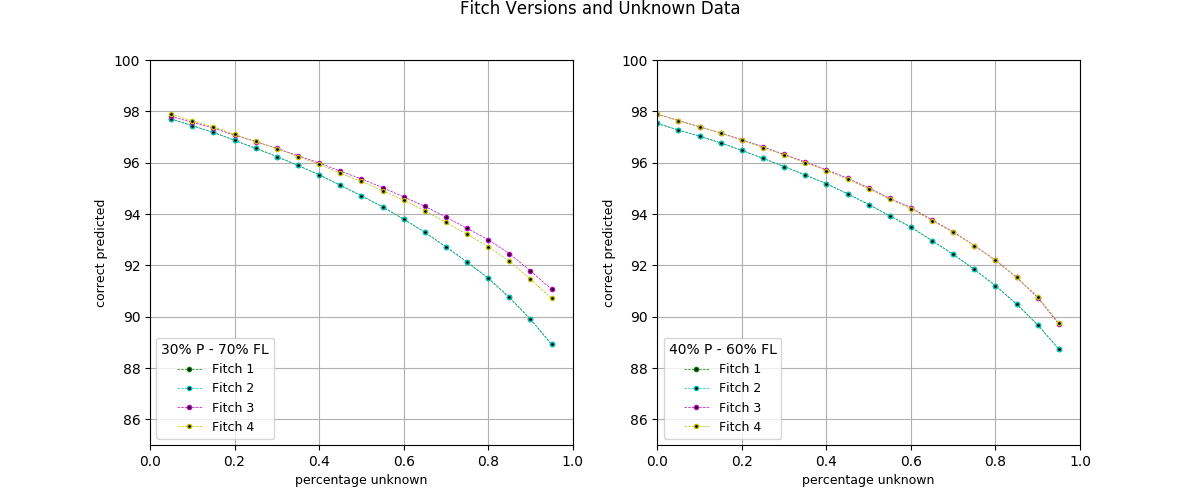
\includegraphics[trim = 24mm 0mm 28mm 14mm, clip, width=\textwidth]{Figures/simulation_fitch_evaluation.png}
        \caption{Test of Fitch Versions. \\
          Each point corresponds to a simulation of 100 trees with 10000 leaf nodes for each proportion 
            (30:70 and 40:60) with equally distributed lack of leaf state information (percentage 
            unknown). The multifurcation probability per node is calculated with: 
            $\frac{1}{max~height(node)}$.}
        \label{fig:Fitch versions}
      \end{figure}
      These four versions are tested in the simulation with 100 trees and 10000 leaf nodes and 
        distributions of 70\% FL to 30\% P and 60\% FL to 40\% P. At 95\% unknown nodes and 95\% of 
        multifurcation of the internal nodes, version 1 is 88.37\%, version 2 is 88.37\%, version 3 is 
        88.4\%, and version 4 is 88.39\% correct.

      There was a more visible difference in the calculations with no equally distributed multifurcation. 
        The probability of forgetting each node was chosen $\frac{1}{max~height(node)}$. Figure 
        \ref{fig:Fitch versions} shows this for different unknown node percentages.

      Therefore, only version 3 is used for all further simulations.

    %---------------------------------------------------------------------------------------------------
    %---------------------------------------------------------------------------------------------------
    \subsection{Sankoff maximum parsimony}
      Maximum parsimony algorithm from Sankoff implemented in the R package \textit{castor} \cite{Louca2017}.
        From this the function \textit{$hsp\_max\_parsimony()$} is used with default settings including
        $transition\_costs="all\_equal"$. \\

  %---------------------------------------------------------------------------------------------------
  %---------------------------------------------------------------------------------------------------
  %---------------------------------------------------------------------------------------------------
  \section{Simulation}
    The simulation compares these different ancestral state reconstruction algorithms with each 
      other. First, different implementations of the Fitch maximum parsimony are collated and then the 
      best of them is compared with the implementation of the Sankoff algorithm of the \textit{castor} 
      package \cite{Louca2017}.

    \begin{figure}[h!]
      \centering
      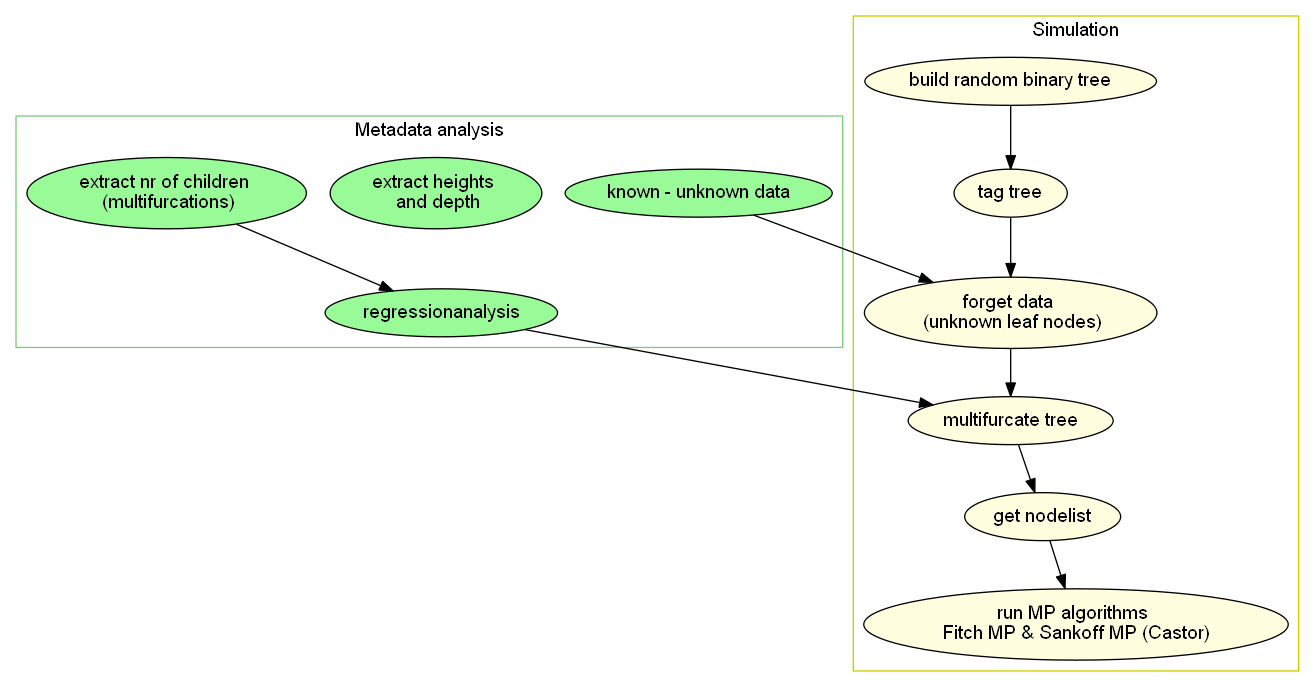
\includegraphics[width=0.95\textwidth]{Figures/Workflow-Simulation.png}
      \caption{A simulation is performed to compare different maximum parsimony algorithms. \\
        The course of the simulation with influence of the metadata analysis from the real data can
          be seen: \\
        (1) Create a phylogenetic tree randomly. (2) Simulate node states for all nodes. (3) 
          'Forget' internal states and some leaf node states. (4) 'Lose' phylogeny information. (5) 
          Make a nodelist for the algorithm. (6) Run algorithms. (7) Evaluate results. \\
        Points 3 and 4 are influenced by metadata of the real-data analysis.}
      \label{fig:Simulation Workflow}
    \end{figure}
    The course of a simulation is shown in Figure \ref{fig:Simulation Workflow}. The individual steps 
      are explained hereinafter.

    A tree is needed to perform a simulation of ancestral state reconstruction. It has to be decided 
      whether to take the real tree or simulate a tree. In this simulation, trees are created randomly, 
      as one can replicate a complete binary phylogentic tree. Thus, there is also the possibility to 
      simulate the multifurcation. \\
    To get a random binary tree, the Phylo package from biopython is used \cite{Cock2009}. They offer 
      a \textit{randomized()} function which returns a BaseTree\footnote{
        \hyperlink{https://github.com/biopython/biopython/blob/master/Bio/Phylo/BaseTree.py}
        {https://github.com/biopython/biopython/blob/master/Bio/Phylo/BaseTree.py};
        Last checked: 22.03.2018.}.

    The next step is to simulate states for all nodes. Here, the influence of the biological  
      \begin{wrapfigure}[21]{r}{0.55\textwidth}
        \centering
        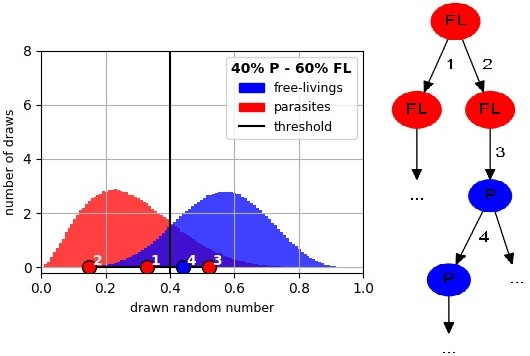
\includegraphics[width=0.55\textwidth]{Figures/40-60_all.jpg}
        \caption{Set node states: Distribution of states (left); traversion through the tree (right). \\
          Start with a free-living root node (FL: red). \\
          (1) + (2) Draw random numbers for its children from the free-living distribution (red), the 
            numbers are under the threshold $\rightarrow$ the nodes are again free-living; go on with 
            the children. \\
          (3) The number drawn is above the threshold. $\rightarrow$ The node state changes to 
            parasitic (P: blue). \\
          (4) Now draw random numbers from the parasite distribution (red) until one number lies under 
            the threshold. Then change back.}
        \label{fig:set node states}
      \end{wrapfigure} 
      parameters as transition probabilities and distributions of states is included.
      
    Since there is no statement about general transition probabilities, these are all set the same: \\
    $\mathcal{P}(FL \rightarrow P) = \mathcal{P}(P \rightarrow FL)$.

    To these distributions different ratios of parasites (P) to free-livings (FL) are simulated with 
      the help of beta distributions and a given threshold:
      \begin{itemize}
        \item 50\% P to 50\% FL,
        \item 40\% P to 60\% FL,
        \item 30\% P to 70\% FL and 
        \item 20\% P to 80\% FL.
      \end{itemize}

    Procedure: The root node is defined as ancestor of all subsequent species and in this case, 
      determined to be free-living. Therefore, the beta distribution for free-living is used at the 
      beginning. A traversion from the root to the leaf nodes sets the states, always pulling out of 
      the current distribution until the randomly drawn number is above the threshold and the new node 
      changes state. Figure \ref{fig:set node states} shows a part of these simulating states and the 
      associated distributions.
    % To ensure that the parameter of the binomial distribution is restricted to the [0,1] interval, it 
    %   is modeled with a beta distribution as in Figure \ref{fig:set node states}. \\

    After traversing through the tree, each state is saved in a nodelist associated with the node 
      identifier which is the OTT from OTL.

    Here begins the simulation of the lack of information, such as the lack of information on topology 
      (multifurcation) and of states of some leaf nodes.
    % = In the simulation, the influence of the multifurcation and missing data in leaf nodes on the 
    %   predictive accuracy of the ancestral state reconstruction algorithms is tested.

    In the real tree, there is usually only information about species living today $\rightarrow$ leaf 
      nodes. And beyond only a small percentage of these. All information about the states of the 
      internal node and one leaf node is removed and stored in another column to the node.

    Last step for the preparation is the multifurcation of the tree. As previously explained, some 
      divisions in the tree are not known, so the real tree is not binary. This multifurcation is 
      simulated by an equally distributed percentage of forgotten internal nodes.
    
    Different percentages of removed information are simulated.
  
    The last step is the evaluation of the results. This is done with a simple difference calculation 
      of the node states. \\
    In the nodelist, the originally simulated states and the newly calculated states are stored for 
      each node ($FL = 0$, $P = 1$). The sum of the differences of the node states gives the distance 
      of the prediction to the original tree.

  %---------------------------------------------------------------------------------------------------
  %---------------------------------------------------------------------------------------------------
  %---------------------------------------------------------------------------------------------------
  \section{Real data analysis}
    For the evaluation of real data results, some statistics are collected and a leave-100-out 
      cross-validation is performed. For this purpose 100 randomly distributed 100 states are left out.

    The statistics are collected over the entire Eukaryota tree and over some subtrees of different 
      taxa. There are known states listed besides predicted states, the predicted root node state 
      specified and origins and losses of parasitism are counted.

    Since Sankoff predicts probabilities for states, we have rounded them to be able to count 
      transitions from free-living (0) to parasitic (1) and vice versa. In each case, a maximum of one 
      changing transition from parent node to child node is counted for the origins (FL $\rightarrow$ 
      P) or losses (P $\rightarrow$ FL).
    
    For the leave-100-out cross-validation, analogous to the missing leaf node states, generalized 
      linear models with binomial regression are compared according to their residuals, based on the 
      "true" / "false" prediction. \\
    Again, in order to compare models of different complexity, the BIC (Bayesian Information Criterion) 
      values are calculated in addition to the residuals. \\
    For all these calculations, the following R functions are used: \textit{glm()}, \textit{anova()} 
      and \textit{BIC()}. \\

  %---------------------------------------------------------------------------------------------------
  %---------------------------------------------------------------------------------------------------
  %---------------------------------------------------------------------------------------------------
  \section{Implementation}
    The complete code is located on GitHub: 
      \hyperlink{github.com/Irallia/IZW-HU-Parasites}{github.com/Irallia/IZW-HU-Parasites}. \\

    Most of the code is written in Python. The analyzes and the use of the \textit{castor} package 
      are partly implemented in R. Some shell scripts are used to execute whole workflows.

%---------------------------------------------------------------------------------------------------
%---------------------------------------------------------------------------------------------------
%---------------------------------------------------------------------------------------------------
%---------------------------------------------------------------------------------------------------
\chapter{Results}
  In the first part of this study, we were able to provide the proof of concept for the Sankoff 
    algorithm to perform an ancestral state reconstruction of the present Eukaryota tree. We will 
    therefore discuss hereinafter how significant the result of this reconstruction is.

  For this reconstruction, we first analyzed our input data. The use of Open Tree of Life (OTL) for
    the tree gives us the greatest approximation to a phylogeny of the Eukaryota. Since such a large
    phylogeny has not been completely dissected, this is only a synthesis of phylogenetic trees with
    a taxonomy as a backbone. Therefore, the tree is far from binary, resulting in a multifurcation 
    of 89.45 \%. However, this is highly variable and therefore the reconstruction is still very 
    good on wide parts of the tree.

  On the other hand, we used the Global Biotic Interactions (GloBI) database to get the state 
    information for the leaf nodes. However, we were able to extract only 2.66\% of the node 
    information from GloBI. However, we found out that there are more data in GloBI that could be 
    taken away with some work.
  
  Next, we consider the limitations of the simulation that led to the choice of the Sankoff 
    algorithm. Our main criticism is that we did not simulate the transition probabilities and 
    estimate an unrealistically high number of transitions (origins and losses). The Sankoff 
    algorithm is very well scored despite this increased difficulty (more transitions means more 
    complex predictions) and its proven feasibility.

  Finally, we analyze the validation of our ancestral state reconstruction results. We will do a 
    statistical analysis from the tree and some selected subtrees and consider the leave-100-out 
    cross-validation. Of these omitted nodes, we predict 98.17\% correctly. \\
    % Here, interested researchers may have to analyze the subtrees that are relevant to them. \\

  %---------------------------------------------------------------------------------------------------
  %---------------------------------------------------------------------------------------------------
  %---------------------------------------------------------------------------------------------------
  \section{Availability of internal nodes and state information}
    As previously presented, we have two types of missing information: unknown states of leaf nodes 
      and multifurcation.

    A tree is multifurcated if there are nodes that have more than two children. A binary tree with 
      $n$ leaf nodes has $n-1$ internal nodes. The present Eukaryota tree of OTL has 2,293,463 leaf 
      nodes and only 241,974 internal nodes, that is:
    $$100-\frac{100}{(2293463-1) \times 241974} \approx 89.45\%$$
      missing internal nodes. This means that there is a lack of information about the underlying 
      phylogeny. Instead of being binary, this tree is highly multifurcated. \\
    \begin{table}[h!]
      \begin{center}
        \begin{tabular}{ |l||r|r| }
          \hline
          \bfseries Subtree of & \bfseries Unknown States & \bfseries Multifurcation \\ 
          \hline \hline
          Eukaryota       & 97.34\%  & 89.45\% \\
          \hline \hline
          Chloroplastida  & 99.14\%  & 89.46\% \\ \hline
          Fungi           & 98.87\%  & 96.97\% \\ \hline
          Metazoa         & 96.44\%  & 87.93\% \\
          \hline \hline
          Apicomplexa     & 86.26\%  & 87.16\% \\ \hline
          Arthropoda      & 97.49\%  & 89.95\% \\ \hline
          Chordata        & 88.59\%  & {\cellcolor{green!50}}66.49\% \\ \hline
          Nematoda        & 89.01\%  & 88.59\% \\ \hline
          Platyhelminthes & {\cellcolor{green!50}}68.73\%  & 80.34\% \\
          \hline \hline            
          Insecta         & 97.11\%  & 90.78\% \\
          \hline  
        \end{tabular}
      \end{center}
      \caption{Examination of subtrees regarding missing information. \\
        The percentage values show the proportion of missing information of: unknown states (missing 
          state information of leaf nodes) and multifurcation (missing internal nodes). \\
        The subtrees are from different taxa: domain (Eukaryota), kingdom (Metazoa, Fungi, 
          Chloroplastida), phylum (Apicomplexa, Nematoda, Chordata, Platyhelminthes) and class 
          (Insecta). \\
        The two by far smallest values are highlighted in green.} 
      \label{table:percentage loss information subtrees} 
    \end{table} \\

    For the present Eukaryota tree with 2,293,463 leaf nodes, 34,869 free-livings and 25,962 parasites 
      are found. This gives
      $$100-\frac{100}{2293463 \times (34860+25962)} \approx 97.34\%$$
      unknown states of leaf nodes.

    We calculated these percentages of missing internal nodes and of missing state information for 
      some subtrees and plotted them in table \ref{table:percentage loss information subtrees}.

    \begin{figure}[h!]
      \centering
      \begin{subfigure}[b]{0.59\textwidth}
        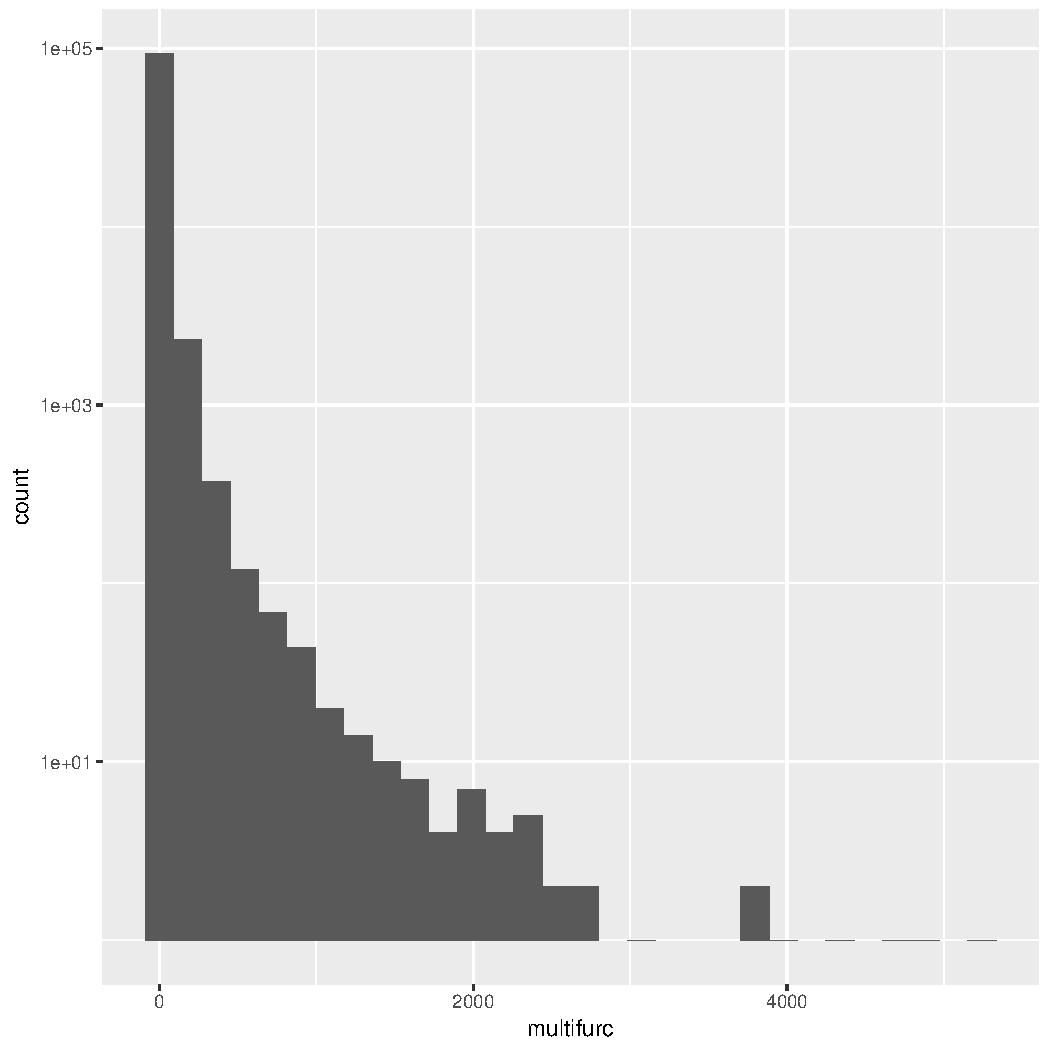
\includegraphics[width=0.9\textwidth]{Figures/multifurc.pdf}
        \caption{Histogram with automatic binwidth. \\ ~}
      \end{subfigure}
      \begin{subfigure}[b]{0.4\textwidth}
        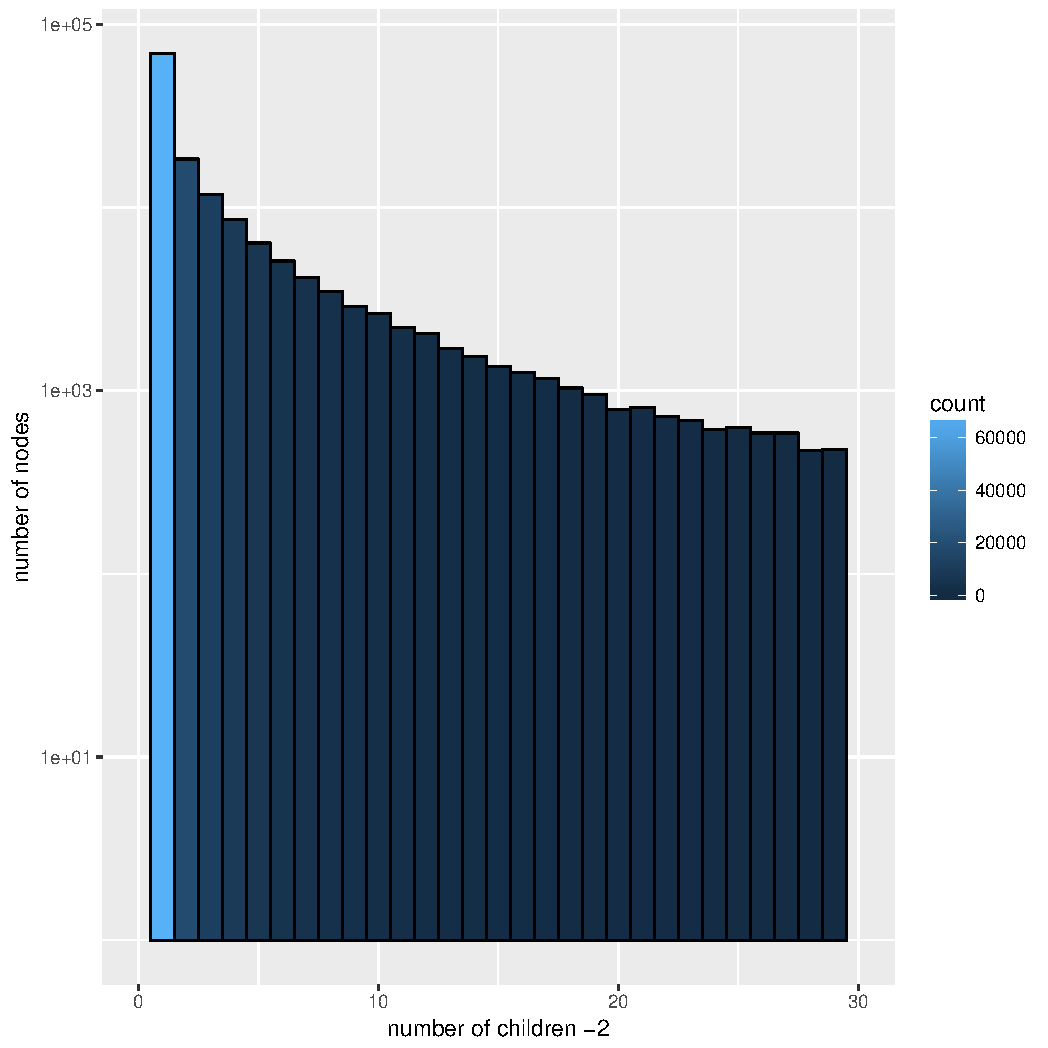
\includegraphics[trim = 0mm 0mm 30mm 0mm, clip, width=0.9\textwidth]{Figures/multifurc_small.pdf}
        \caption{Histogram with $binwidth = 1$. Higher multifurcation than 30 has been cut off. \\
          light blue: binary; \\ dark blue: multifurcation}
      \end{subfigure}
      \caption{Histograms showing the multifurcation of the internal nodes of the synthesis tree. \\
        For each node, the number of children (degree $-1$) is collected. A node is multifurcated if it
        has more than two children, so we deducted two from each number of children. The two histograms 
        show the number of children $-2$ on the x-axis with log scale and the number of nodes with this 
        amount on the y-axis.}
      \label{fig:childrenOfNodes}
    \end{figure}

    The multifurcation affects only the internal nodes. We collected the number of children (degree $-1$) 
      of these nodes and than subtract two of each value (because a node with two children is binary). 
      That means this value describes the number of nodes which we have lost from the real (binary) 
      phylogenetic tree. We plotted this in two histograms, see figure \ref{fig:childrenOfNodes}. It can 
      be recognized that we are very far from a binary tree.

    %---------------------------------------------------------------------------------------------------
    %---------------------------------------------------------------------------------------------------
    \subsection{Comparison of different models for multifurcation}
      For the regression analysis of the multifurcation we set up several generalized linear models that 
        could describe multifurcation.

      In doing so, we allowed the different influence of the taxa and the heights and depths of a node 
        to be included. From this we got 9 times 4 models of different complexity levels (first row) and 
        the associated BIC values (table \ref{table:BIC multifurcation}).

      \begin{table}[h]
        \begin{center}
          \begin{tabular}{ |l|r|r|r|r| }
            \hline
            \bfseries Model / Taxa & \bfseries Kingdom & \bfseries Phylum & \bfseries Class & \bfseries Order \\
            \hline \hline
            multifurcation $\sim$ taxa & 8273333 & {\cellcolor{green!15}}7937828 & {\cellcolor{green!20}}7842157 & {\cellcolor{green!30}}7644249 \\
            multifurcation $\sim$ taxa & 8257680 & {\cellcolor{green!15}}7922207 & {\cellcolor{green!20}}7826490 & {\cellcolor{green!35}}7574154 \\
            \hline
            multifurcation $\sim$ taxa + depth & 8273318 & {\cellcolor{green!15}}7934322 & {\cellcolor{green!20}}7839364 & {\cellcolor{green!35}}7539999 \\
            multifurcation $\sim$ taxa + max.height & {\cellcolor{green!15}}7993515 & {\cellcolor{green!25}}7749121 & {\cellcolor{green!30}}7661817 & {\cellcolor{green!40}}7416211 \\
            multifurcation $\sim$ taxa + min.height & 8251211 & {\cellcolor{green!20}}7875521  & {\cellcolor{green!25}}7778327 & {\cellcolor{green!35}}7516883 \\
            multifurcation $\sim$ taxa + mean.height & {\cellcolor{green!20}}7825417 & {\cellcolor{green!30}}7644249 & {\cellcolor{green!35}}7572474 & {\cellcolor{green!45}}7340741 \\
            \hline
            multifurcation $\sim$ taxa * depth & 8235932 & {\cellcolor{green!20}}7836755 & {\cellcolor{green!25}}7757688 & {\cellcolor{green!45}}7383808 \\
            multifurcation $\sim$ taxa * max.height & {\cellcolor{green!15}}7963438 & {\cellcolor{green!30}}7693555 & {\cellcolor{green!30}}7614820 & {\cellcolor{green!45}}7335338 \\
            multifurcation $\sim$ taxa * min.height & 8214030 & {\cellcolor{green!20}}7808940 & {\cellcolor{green!30}}7690618 & {\cellcolor{green!45}}7336627\\
            multifurcation $\sim$ taxa * mean.height & {\cellcolor{green!25}}7768360 & {\cellcolor{green!35}}7536296 & {\cellcolor{green!50}}7484953 & {\cellcolor{green!50}}7206369 \\
            \hline
          \end{tabular} 
        \end{center}
        \caption{BIC values of the multifurcation models. \\
          These models are created with the R function \textit{glm()} and compared with the \textit{BIC()} 
            function. These results are the listed BIC values, presented in a heatmap colorization.}
        \label{table:BIC multifurcation} 
      \end{table}
      Within every complexity class it can be seen that the mean height gives the best additional factor.
        Despite higher complexity, the BIC values are getting smaller from model to model, meaning that 
        the finest model available here is also the best one of these. Lower order taxa e.g. family are 
        computationally too expensive to calculate.

      The model \textit{multifurcation $\sim$ order * mean.height} turns out to be the best of our models, 
        whereby it is possible that e.g. \textit{multifurcation $\sim$ family * mean.height} is better. \\

    %---------------------------------------------------------------------------------------------------
    %---------------------------------------------------------------------------------------------------
    \subsection{Comparison of different models for missing state information}
      Next to the problem of the multifurcation of the tree is the little interaction data that we have 
        for the species. For the ancestral state reconstruction, we need information about the states 
        (free-living or parasite) of the leaf nodes.
        
      The Eukaryota synthesis tree has 293,463 leaf nodes. The GloBI database has 5,346,414 interactions 
        (at 29.01.2018). Out of this data we received 51,337 free-living species and 47,332 parasite 
        species for the whole tree of life. For the Eukaryota we could determine 25,962 and 34,860 
        species as parasites and free-living. With 2,293,463 leaf nodes we still have about 97.34\% 
        unknown leaf nodes.
      
      We also compared different models in terms of their BICs (table: \ref{table:BIC unknown information}). \\ 
      \begin{table}[h!]
        \begin{center}
          \begin{tabular}{ |l|r|r|r|r| }
            \hline
            \bfseries Model / Taxa & \bfseries Kingdom & \bfseries Phylum & \bfseries Class & \bfseries Order \\
            \hline \hline
            multifurcation $\sim$ taxa & {\cellcolor{green!15}}545799 & {\cellcolor{green!35}}500004 & {\cellcolor{green!45}}485121 & {\cellcolor{green!45}}484681 \\
            \hline
            multifurcation $\sim$ taxa + depth & {\cellcolor{green!15}}544862 & {\cellcolor{green!40}}493808 & {\cellcolor{green!45}}481869 & {\cellcolor{green!50}}478851 \\
            \hline
            multifurcation $\sim$ taxa * depth & {\cellcolor{green!15}}544179 & {\cellcolor{green!45}}489845 & {\cellcolor{green!45}}481494 & {\cellcolor{green!50}}478188 \\
            \hline
          \end{tabular} 
        \end{center}
        \caption{BIC values unknown state information models. \\
          These models are created with the R function \textit{glm()} and compared with the 
            \textit{BIC()} function. This results in the listed BIC values, presented in a heatmap colorization.}
        \label{table:BIC unknown information} 
      \end{table}

      It also follows from this table that the most complex model is the best. In general, the BIC 
        values are smaller than those of the multifurcation models. The modeling here is thus better.
        Again, the calculation of finer models (e.g. family) was too expensive.

      These missing data modeling results could be used to improve the simulated data. \\

  %---------------------------------------------------------------------------------------------------
  %---------------------------------------------------------------------------------------------------
  %---------------------------------------------------------------------------------------------------
  \section{Influence of different parameters on the prediction}
    As presented, we compare two methods in our simulation to their prediction accuracy: Fitch and 
      Sankoff.

    First, we tested different distributions of parasites to free-livings including threshold (first 
      column).We observe: the more balanced the percentages of free-livings and parasites, the worse 
      the prediction of the algorithms (second and third column). It can be seen that the predictive 
      power of Sankoff is always greater or equal to the percentage of free-living distribution, and 
      therefore more accurate than guessing.

    On the other hand, we examined the influence of missing internal nodes (ridge of multifurcation) 
      and missing leaf node information (unknown leaf nodes). Both factors have a relatively linear 
      influence on the Sankoff method. Fitch, on the other hand, breaks significantly in his 
      prediction from about 70\% unknown leaf nodes or mutifurcation.

    Figure \ref{fig:influence of unknown data} shows the results of examining various parameters.

    \begin{figure}[h!]
      \centering
      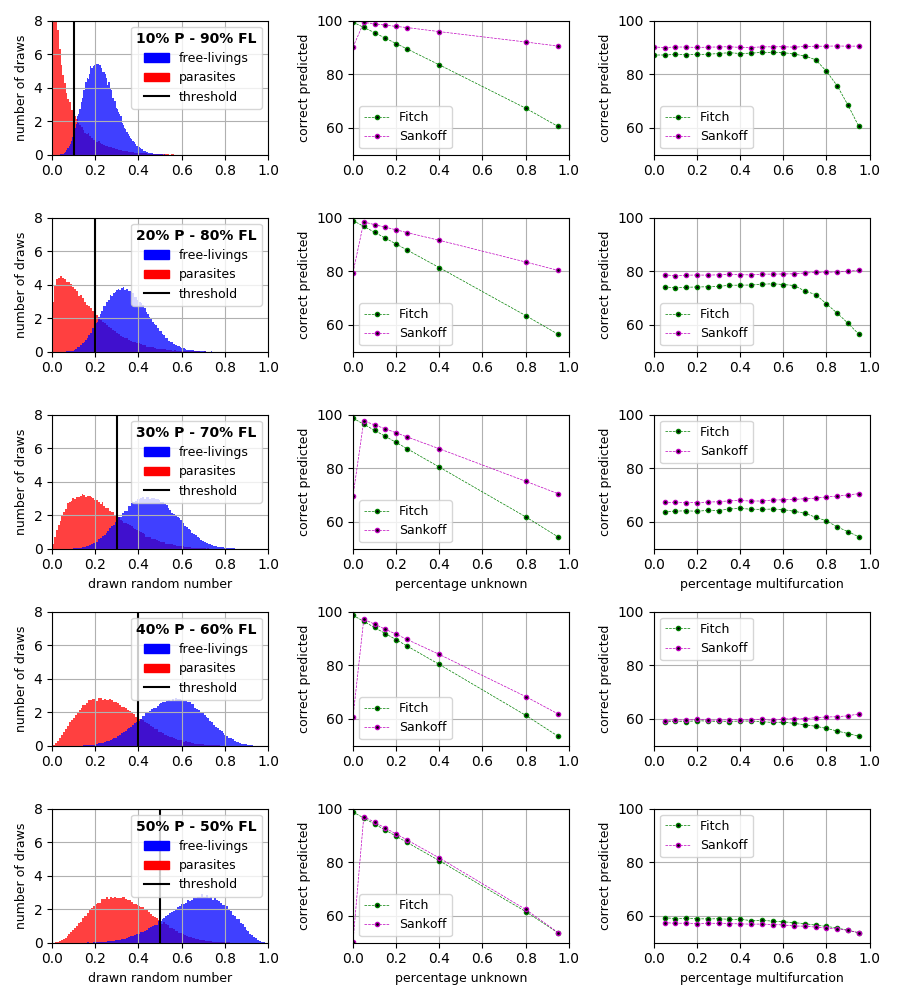
\includegraphics[trim = 0mm 108mm 0mm 0mm, clip, width=\textwidth]{Figures/simulation_evaluation_1.png}
    \end{figure}
    \begin{figure}[h!]
      \centering
      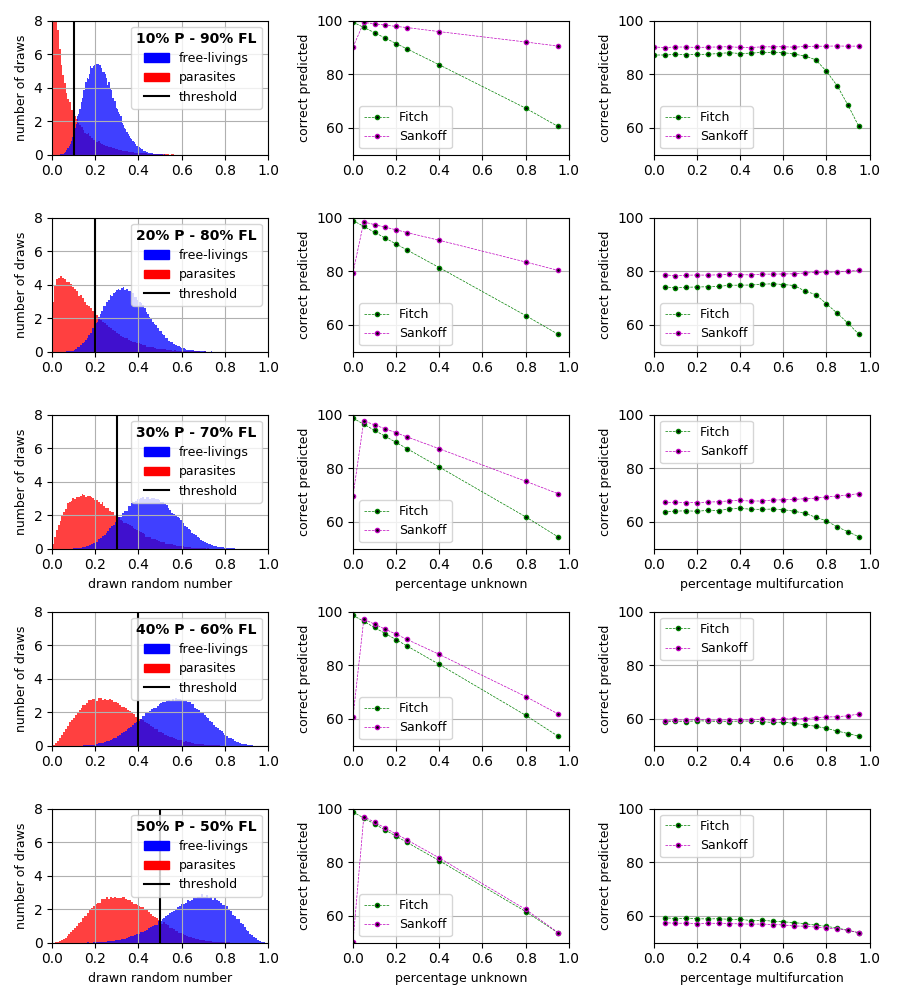
\includegraphics[trim = 0mm 0mm 0mm 150mm, clip, width=\textwidth]{Figures/simulation_evaluation_1.png}
      \caption{Influence of unknown data to prediction. \\
        The first column describes the distributions of free-livings and parasites with a given 
          threshold for the respective simulations to the right. Note, these distributions are chosen 
          to form the specified proportions with the threshold, ignoring the number of state changes. \\
        The middle column investigates the influence of the unknown states, the right the influence of
          the strength of the multifurcation. \\
        The y-axes indicate the percentage of correctly predicted states (including known states). The 
          x-axis describes the percentage of forgotten states or missing internal nodes. \\
        Each point corresponds to the average of 100 simulations, each with 10,000 leaf nodes. \\
        For the middle column we set the strength of the multifurcations to 0.95\%, similar to the 
          real data and in the right column the amount of the unknowns to 0.95\%, also similar to the 
          real data.}
      \label{fig:influence of unknown data}
    \end{figure}

    Since we have a lot of missing data in most subtrees (both internal nodes and state information), 
      the Sankoff gives a better prediction and is thus used for the real data analysis. \\

  %---------------------------------------------------------------------------------------------------
  %---------------------------------------------------------------------------------------------------
  %---------------------------------------------------------------------------------------------------
  \section{Results of the real data analysis created with Sankoff}
    This section is about evaluating the prediction of real data using the Sankoff method and is 
      divided into two subsections.

    First comes the analysis of some statistics on the predicted states, with the result that we 
      predict a total of significantly more free-livings than parasites despite almost 50:50 
      distributed input states, and second, we present the leave-100-out cross-validation results. This 
      revealed that we predicted approximately 98.17\% correct with a small variance.

    %---------------------------------------------------------------------------------------------------
    %---------------------------------------------------------------------------------------------------
    \subsection{Statistics on predicted states}
      In the entire Eukaryota tree we start with 57.31\% free-living species and 42.69\% parasites. The 
        prediction yields 80.98\% free-livings 0.31\% undefinable and 18.71\% parasites. In addition, 
        there are 462 origins of parasitism and 369 losses distributed throughout the tree, with the 
        root node predicted to be parasitic. We have predicted significantly more free-livings than 
        parasites, but parasitism has prevailed to the root node.
      
      In table \ref{table:results of some selected taxa} we compare different subtrees of different taxa 
        on these prediction results.
      
      Similar to the Eukaryota it is with the Metazoa subtree, which accounts for most of the Eukaryota 
        (179,944 internal and 1,491,012 leaf nodes). However, the root node here is no longer calculated 
        as parasitic but still as indefinable.

      Strongly parasitic subtrees are, for example, the Apicomplexa, the Nematoda and the Platyhelminthes. 
        For all three, the prediction is at a similar proportion between input values of the states and 
        predicted states. In the Apicomplexa with 99.61\% known parasitic states, 99.95\% parasites 
        were predicted. The same applies to the Chordata, only that these mainly consist of free-living 
        species.
      
      % \tiny	\scriptsize \footnotesize \small \normalsize \large \Large \LARGE \huge \Huge
      \begin{table}
        \begin{center}
          \hspace*{-0.5cm}\begin{tabular}
              {|>{\scriptsize}c|>{\scriptsize}l|>{\scriptsize}r|>{\scriptsize}r||>{\scriptsize}r|>{\scriptsize}r||
                >{\scriptsize}r|>{\scriptsize}r|>{\scriptsize}r||>{\scriptsize}r|>{\scriptsize}r|>{\scriptsize}r| }
            \hline
            \multirow{3}{*}{\rot{\bfseries $\leftarrow$ Taxa}}
            & & \multicolumn{2}{>{\scriptsize}c||}{\bfseries number of}
                & \multicolumn{2}{>{\scriptsize}c||}{\bfseries known states} & \multicolumn{3}{>{\scriptsize}c||}{\bfseries final states}
                & \bfseries Root & \bfseries \#origins & \bfseries \#losses \\
            & \bfseries Subtree & \bfseries internal & \bfseries leaf & \bfseries FL & \bfseries P
                & \bfseries [0, 0.5) & \bfseries 0.5 & \bfseries (0.5, 1]
                & \bfseries node & \multicolumn{2}{>{\scriptsize}c|}{\bfseries (with rounding)} \\
            & \bfseries & \multicolumn{2}{>{\scriptsize}c||}{\bfseries nodes} & &
                & \bfseries FL & & \bfseries P 
                & \bfseries state & \bfseries FL $\rightarrow$ P & \bfseries P $\rightarrow$ FL \\
            \hline \hline
            \parbox[c][7mm][c]{1mm}{\multirow{2}{*}{\rot{\bfseries Domain~}}}
            & Eukaryota & 241974 & 2293463      & 34860 & 25962     & 2053212 & 7775 & 474450     & 1 & 462 & 369 \\
            & & &                               & 57.31\% & 42.69\% & 80.98\% & 0.31\% & 18.71\%  & P & & \\
            \hline \hline
            \parbox[c]{1mm}{\multirow{6}{*}{\rot{\bfseries Kingdom}}}
            & Chloroplastida & 43486 & 416478   & 3519 & 77         & 410795 & 4182 & 1501        & 0.5 & 97 & 222 \\
            & & &                               & 97.86\% & 2.14\%  & 98.63\% & 1.00\% & 0.36\%   & & & \\ \cline{2-12}
            & Fungi & 9534 & 31457              & 577 & 2983        & 38520 & 5723 & 266463       & 0 & 42 & 2 \\
            & & &                               & 16.21\% & 83.79\% & 12.40\% & 1.84\% & 85.76\%  & FL & & \\ \cline{2-12}
            & Metazoa & 179944 & 1491012        & 30758 & 22373     & 1329065 & 25535 & 136412    & 0.5 & 321 & 129 \\
            & & &                               & 57.89\% & 42.11\% & 89.14\% & 1.71\% & 9.15\%   & & & \\
            \hline \hline
            \parbox[c]{1mm}{\multirow{10}{*}{\rot{\bfseries Phylum}}}
            & Apicomplexa & 239 & 1863          & 1 & 255           & 1 & 0 & 1862                & 1 & 0 & 1 \\
            & {\tiny (Chloroplastida)\par} & &  & 0.39\% & 99.61\%  & 0.05\% & 0\% & 99.95\%      & P & & \\ \cline{2-12}
            & Arthropoda & 120479 & 1198981     & 18912 & 11141     & 1100822 & 22478 & 76064     & 0 & 281 & 108 \\
            & {\tiny (Metazoa)\par} & &         & 62.93\% & 37.07\% & 91.78\% & 1.87\% & 6.34\%   & FL & & \\ \cline{2-12}
            & Chordata & 30761 & 91785          & 10451 & 18        & 91759 & 0 & 26              & 0 & 12 & 1 \\
            & {\tiny (Metazoa)\par} & &         & 99.83\% & 0.49\%  & 99.97\% & 0\% & 0.03\%      & FL & & \\ \cline{2-12}
            & Nematoda & 3437 & 30127           & 21 & 3289         & 1746 & 1196 & 27185         & 1 & 2 & 11 \\
            & {\tiny (Metazoa)\par} & &         & 0.63\% & 99.37\%  & 5.79\% & 3.97\% & 90.23\%   & P & & \\ \cline{2-12}
            & Platyhelminthes & 4459 & 22683    & 7 & 7086          & 175 & 0 & 22508             & 0 & 0 & 5 \\
            & {\tiny (Metazoa)\par} & &         & 0.10\% & 99.9\%   & 0.77\% & 0\% & 99.23\%      & P & & \\
            \hline \hline 
            \parbox[c]{1mm}{\multirow{2}{*}{\rot{\bfseries Class~}}}
            & Insecta & 91256 & 989572          & 17841 & 10734     & 1022747 & 976 & 57105       & 0 & 245 & 77 \\
            & {\tiny (Arthropoda)\par} & &      & 62.44\% & 37.56\% & 94.63\% & 0.09\% & 5.28\%   & FL & & \\ 
            \hline
          \end{tabular} 
        \end{center}
        \caption{Results of some selected taxa (subtrees). \\
          (1 + 2) subtree taxa and name; 
          (3 + 4) number of internal nodes and leaf nodes; 
          (5 + 6) number or percentage of known states; 
          (7 - 9) number or percentage of predicted states; 
          (10) predicted state of the root node of the subtree; 
          (11 + 12) origins and losses with rounded states.}
          \label{table:results of some selected taxa}
      \end{table}

~ \\

      Weinstein and Kuris have been searching for origins of parasitism in Animalia \cite{Weinstein2016}. 
        They identified 223 parasitic origins: 223 in Metazoa $\supset$ 143 in Arthropoda $\supset$ 87 
        in Insecta. In the last columns of the table \ref{table:results of some selected taxa} we see 
        that we found more origins than Weinstein: 321 in Metazoa $\supset$ 281 in Arthropoda $\supset$ 
        245 in Insecta and on top of that some losses: 129 in Metazoa $\supset$ 108 in Arthropoda 
        $\supset$ 77 in Insecta. The origins and losses calculated by Sankoff are thus closer to the 
        leaves in the tree.

    %---------------------------------------------------------------------------------------------------
    %---------------------------------------------------------------------------------------------------
    \subsection{Leave-100-out cross-validation}
      For a further validation of our results, we carried out a leave-100-out cross-validation. In order 
        to achieve about 15\% of the 60,871 input node states with a validation, we randomly left out 
        100 states 100 times. Omitting smaller amounts of states up to leave-one-out had too much 
        computational effort.
        
      Of these 10,000 nodes, 9,238 are unique. From the unique nodes, we predicted approximately 
        98.17\% correct and thus 1.82\% wrong, with duplicate draws always having the same prediction. 
        The associated variance is 0.017, which means that no large amounts of input states have to be 
        omitted.
      
      We have again considered how this data can best be modeled to compare whether there is a lot 
        of variability in the taxa and whether the depth is an influencing factor over our prediction. 
        The influence of the taxa (kingdom, phylum, class) and the depth of the leaf nodes is remodeled 
        and the BICs compared (table \ref{table:BIC cross-validation}). Lower order taxa than classes 
        (e.g. order) are computationally too expensive to calculate.

      % \todo{table for these numbers?}
      % 100/(25962+34860)*10000 = 16.44
      % 100/(25962+34860)*9238 = 15.19
      % 10000 nodes 9238 unique
      % 9060 nodes $\approx 98.17\%$ correctly predicted
      % 169 ($\approx 1.82\%$) wrongly predicted
      % variance is 0.017

      \begin{table}[h]
        \begin{center}
          \begin{tabular}{ |l|r|r|r| }
            \hline
            \bfseries Model / Taxa & \bfseries Kingdom & \bfseries Phylum & \bfseries Class \\% & Order \\
            \hline \hline
            correctly predicted $\sim$ taxa & 117936 & {\cellcolor{green!40}}112242 & {\cellcolor{green!50}}111733 \\% & XXXXX \\
            \hline
            correctly predicted $\sim$ taxa + depth & 117776 & {\cellcolor{green!50}}111304 & {\cellcolor{green!50}}111273 \\% & XXXXX \\
            \hline
            correctly predicted $\sim$ taxa * depth & 117709 & {\cellcolor{green!50}}111262 & {\cellcolor{green!30}}113135 \\% & XXXXX \\
            \hline
          \end{tabular} 
        \end{center}
        \caption{BIC values of cross-validation prediction models. \\
          These models are created with the R function \textit{glm()} and compared with the 
            \textit{BIC()} function. This results in the listed BIC values, presented in a heatmap colorization.}
        \label{table:BIC cross-validation} 
      \end{table}

      The BIC values this time did not prove that the finest model is the best. Of our calculated models, 
       \textit{correctly predicted $\sim$ phylum * depth} has the smallest value.

      We examined the influence of the omitted data on the prediction. On average, about twice as many 
        leaf nodes are predicted differently. %\color{red}The variance is very high. This means that 
        % we have a high degree of dispersion and thus a stochastic situation exists. It also describes 
        % the width of the present probability function. The standard deviation is about five times as 
        % high as the number of omitted nodes, so the variability is quintupled. \color{black} 
        Table \ref{table:statistics cross-validation} shows these results. \\
      \begin{table}[h!]
        \begin{center}
          \begin{tabular}{ |cl||r|r|r|r|r| }
            \hline
            & & \bfseries min & \bfseries max & \bfseries mean & \bfseries variance ($\sigma^2$) & $\sigma$ \\
            \hline \hline
            \multirow{3}{*}{\bfseries distance} & \bfseries all     & 0 & 3587.70 & 224.96 & 313650.61 & 560.05 \\
            & \bfseries leaf nodes                                  & 0 & 3021.12 & 208.69 & 248103.38 & 498.10 \\
            & \bfseries internal nodes                              & 0 & 566.58 & 16.28 & 4927.95 & 70.20 \\ \hline
            % \multirow{3}{*}{\bfseries lost} & \bfseries all states  & 100 & 100 & 100 & 0 & 0 \\
            % & \bfseries FL states                                   & 44 & 66 & 57.25 & 19.50 & 4.42 \\
            % & \bfseries P states                                    & 34 & 56 & 42.75 & 19.50 & 4.42 \\
            % \hline
          \end{tabular}
        \end{center}
        \caption{Statistics about the leave-100-out cross-validation \\
          The distance between original and new states is calculated using the Euclidean metric. This 
            is summed over all states, all leaf node states and all internal node states.}
          % The lower half of the table describes the distribution of the 'lost' states between parasites 
            % (P) and free-livings (FL).}
        \label{table:statistics cross-validation}
      \end{table}

%---------------------------------------------------------------------------------------------------
%---------------------------------------------------------------------------------------------------
%---------------------------------------------------------------------------------------------------
%---------------------------------------------------------------------------------------------------
\chapter{Discussion}
  This chapter is about how trustworthy our result of the ancestral state reconstruction of the 
    Eukaryota tree is and how good our simulation is in order to make statements about the predictive 
    power of the applied Sankoff algorithm.

  We pursued this question in various investigations and yet, of course, further possibilities for 
    improvement remain. Despite these improvement opportunities, our reconstruction gives a first 
    good assessment of the whole tree.

  In the first part of this work, we were able to provide the proof of concept for the Sankoff 
    algorithm to perform an ancestral state reconstruction of the present Eukaryota tree. Hereinafter, 
    
    we will first discuss the data situation and the simulation that led to the selection of the 
    Sankoff algorithm, followed by a discussion about the significance of the result of this 
    reconstruction.

  We evaluated our ancestral state reconstruction and the relational state prediction using a 
    leave-100-out cross-validation. In addition, in this chapter, we will take a closer look at some 
    subtrees and discuss their credibility from a biological perspective.

  %---------------------------------------------------------------------------------------------------
  %---------------------------------------------------------------------------------------------------
  %---------------------------------------------------------------------------------------------------
  \section{Data situation}
    The used Eukaryota synthesis tree from OTL \cite{Hinchliff2015} has 241,974 internal nodes and 
      293,463 leaf nodes. In addition, we could specify 25,962 parasitic and 34,860 free-living 
      species from GloBI \cite{Poelen2014}. \\
    This gives us a high number of missing internal nodes (high multifurcation) and a low number of 
      states of the leaf nodes in the entire tree.
    We suspect that this lack of information is not equally distributed in both cases. We conclude 
      this from various observations:

    For one, there were a few subtrees of higher ranks whose information share was much greater. In 
      the Chordata there is only 66.49\% multifurcation and in the Platyhelminthes only 68.73\% 
      missing state information.

    Furthermore, we know that OTL is a synthesis of 819 phylogenetic trees. This suggests that just 
      these parts of the tree are very well resolved and the remainder consists only of the rough 
      taxonomy. For a review of this underlying taxonomy, we have compiled a list of all taxa and 
      plotted them in relation to their distribution (see appendix section \ref{sec:appendix - otl analysis}). 
      In this list, the number of nodes in the tree corresponding to a taxonomic rank is tabulated.

    % The investigation of the taxonomy revealed that the OTL tree has three kingdoms: Chloroplastida, 
    %   Metazoa, Fungi, 53 phyla, 195 classes and 924 orders. \\
    % Since the analysis of the tree is not part of this work, it should be mentioned here that, 
    %   according to recent findings, this is not complete and we lack some taxa in every rank. For 
    %   example, Cavalier-Smith says that one distinguishes between seven and nine kingdoms 
    %   \cite{CavalierSmith1981}. \\
    
    From GloBI we received very little information about leaf node states compared to their quantity 
      in the Eukaryota tree. Nevertheless, the prediction of the leave-100-out cross-validation was 
      very good. This also leads to the conclusion that the information is very clustered.

    As a last point, we would like to cite the modeling of the missing information. The fact that this 
      gets better, the lower the taxa (smaller subtrees) we are looking at, also indicates a high 
      variability of the data.

    We would like to mention a few other aspects of the GloBI database here. Of course, such large 
      data sets are flawed. We found some misinformation and were able to report some of these 
      directly to GloBI. We also noticed that there is some unused information in GloBI. We found some 
      source species and target species without OTT identifiers. Since we currently use only OTT 
      identifiers, we could not use this information. At this point there is thus the possibility to 
      use more of the existing data, if one performs a matching with the other identifiers.

  %---------------------------------------------------------------------------------------------------
  %---------------------------------------------------------------------------------------------------
  %---------------------------------------------------------------------------------------------------
  \section{Simulation} \label{sec:discussion - simulation}
    The aim of the simulation is to test the influence of various unknown or uncertain parameters on 
      some selected algorithms in order to test the credibility of the prediction of these for the 
      given problem.

    We assume that different parasite types have different transition probabilities. It is therefore 
      difficult to establish a common distribution across the Eukaryota tree. Based on the estimates 
      of Windsor \cite{Windsor1998}, we have assumed a distribution of 40\% parasites to 60\% 
      free-livings in this study. As a result of the diversity of parasites and the lack of 
      generalizations, we have stated that 
      $\mathcal{P}(FL \rightarrow P) = \mathcal{P}(P \rightarrow FL)$. But it is also reasonable to 
      assume that in general $\mathcal{P}(FL \rightarrow P) > \mathcal{P}(P \rightarrow FL)$, because 
      a reverse mutation is usually less likely. However, one would have to determine how much this 
      difference is and thus discuss another parameter.
    
    In the simulation, we found that this combination has a significant influence on the predictive 
      power of the algorithms. We have adapted the combination of distributions and threshold to a 
      high probability of achieving the given proportions on initial attempts. However, this means 
      that we prefer high transition probabilities for both transitions and thus the simulated trees 
      have a large number of transitions. It can be assumed that this may not correspond to the real 
      data and thus means a limitation of our simulation. Furthermore we assume that with a lower 
      number of state changes, the predictive power of both algorithms would be even better, thus this 
      limitation is probably not very restrictive. At this point it would be possible to test other 
      distributions with equal threshold values. This would be more computationally expensive, but 
      would result in fewer transitions.

    % With these further simulations you could find out if the issue of distributions plays a big role. 
    %   Conversely, one could estimate possible distributions based on the data location in the tree. 
    %   However, this is likely to be very difficult given the poor data. For this reason, we have 
    %   decided in this work to accept very general values and not to speculate much. \\

    The used \textit{castor} package \cite{Louca2017} offers the possibility to enter different 
      transition probabilities, so with information about these probabilities, one might be able to 
      improve the prediction here.

  %---------------------------------------------------------------------------------------------------
  %---------------------------------------------------------------------------------------------------
  %---------------------------------------------------------------------------------------------------
  \section{Biological view}
    We have selected some phyla (subtrees) to evaluate our results selectively 
      from the biological point of view: Chordata, Nematoda, Platyhelminthes and Apicomplexa. Various 
      factors such as the distribution of existing input data about parasites and free-livings, 
      erroneous input data from GloBI, and the amplification of these errors due to multifurcation 
      play an important role, which becomes clear in these examples.

    The accuracy of our results stands and falls with the presence and the correctness of the data of 
      GloBI. Errors that result from incorrect data can be amplified by incorrect prediction of unknown 
      species and can be reversed in order to improve the data situation of GloBI. Since we look at 
      such large trees we can not expect to know all the parasites, so we look at individual positives. 
      They are positive in the sense that the majority have the opposite state.

    In contrast to the other phyla examined, the phylogeny in the Chordata is more pronounced (less 
      multifurcation). This leads to a lower variance of errors, which is reflected in the results. 
      There are 18 parasites as input data and only 8 more are predicted. The Chordata mostly consist 
      of free-living species, so this seems credible. We started with 99.83\%  species and predicted
      99.97\% species as free-living (including already known nodes). For a detailed view we created 
      and described a tree with all known and predicted parasites (see appendix 
      \ref{sec:parasites in chordata}).

    The Apicomplexa are a parasitic phylum. We found only one input organism: \textit{Stemonitis fusca} 
      is a free-living species. It is listed in GloBI as being parasitized by Nectria candicans and 
      Nectriopsis sporangiicola\footnote{
        \hyperlink{https://www.globalbioticinteractions.org/?interactionType=parasiteOf&targetTaxon=Stemonitis\%20fusca}
        {https://www.globalbioticinteractions.org/?interactionType=parasiteOf\&targetTaxon=Stemonitis\%20fusca};
        Last checked: 22.03.2018.
      }. The algorithm has not predicted new free-livings.

    Most species of Platyhelminthes (flatworms) are parasites, although there are also free-living, 
      predatory feeding species. These are summarized in the Turbellaria, while the parasites are 
      divided into three other classes \cite{Ax1961}. This also corresponds to our observations. There 
      is one class (Rhabditophora) that contains all but one single exception of free-living species 
      of this phylum, which includes the Turbellaria. For the Platyhelminthes we have proportionally 
      more state information for the leaf nodes compared to the other considered subtrees. We start 
      with 0.1\% free-livings and predicted 0.77\% as free-living species.

    The Nematoda are more complicated. Large parts of Nematoda are free-living, but we found only 
      5.32\% of them. Blaxter and Koutsovoulos estimate the order of 25,000 parasites in the Nematoda 
      and speak of 18 independently arosen parasites in Nematoda \cite{Blaxter2015}. We assume that 
      the parasites have been much more studied and thus we start with only 0.63\% free-living species. 
      Against such a shifted data situation, the algorithm is almost powerless to make correct 
      predictions. And yet the percentage has increased to 5.34\%.

    The root node of the Nematoda is predicted as a parasite and so we received 11 losses of parasitism 
      and only 2 origins in this phylum. If we assume that the root node of Nematoda is free-living, 
      then some losses would have to turn around and become Origins. So it could be that we end up 
      with a similar size as Blaxter and Koutsovoulos \cite{Blaxter2015}.

  %---------------------------------------------------------------------------------------------------
  %---------------------------------------------------------------------------------------------------
  %---------------------------------------------------------------------------------------------------
  \section{Conclusion}

    From the simulation, we can conclude that we predict about 60\% of the nodes in the present data 
      situation correctly. The leave-100-out cross-validation even showed that we predict the omitted 
      nodes to be 98.17\% percent correct.

    This allows for the assumption that the data is grouped and not uniformly distributed and thus 
      smaller subtrees are present in which data are to be found in the simulation with smaller 
      multifurcation and smaller value for unknown nodes. This is also confirmed by our statistical 
      and biological analysis of the considered subtrees: Chordata, Nematoda, Platyhelminthes and 
      Apicomplexa.

    However, it follows that the ancestral states' data in the direction of root node are probably 
      particularly unreliable. This makes the localization of origins in direction of the root node 
      difficult. The question remains, how much this affects the estimation of the number of origins. 
      Our comparison with the paper from Weinstein and Kuris \cite{Weinstein2016} an with Blaxter and 
      Koutsovoulos \cite{Blaxter2015} showed similar numbers of origins in some subtrees, which 
      leaves us with optimism.

%---------------------------------------------------------------------------------------------------
%---------------------------------------------------------------------------------------------------
%---------------------------------------------------------------------------------------------------
\bibliography{bibliographie}

%---------------------------------------------------------------------------------------------------
%---------------------------------------------------------------------------------------------------
%---------------------------------------------------------------------------------------------------
\chapter{Appendix}
  %---------------------------------------------------------------------------------------------------
  %---------------------------------------------------------------------------------------------------
  \section{Methods overview}
    % \begin{figure}[h!]
    %   \centering
    %   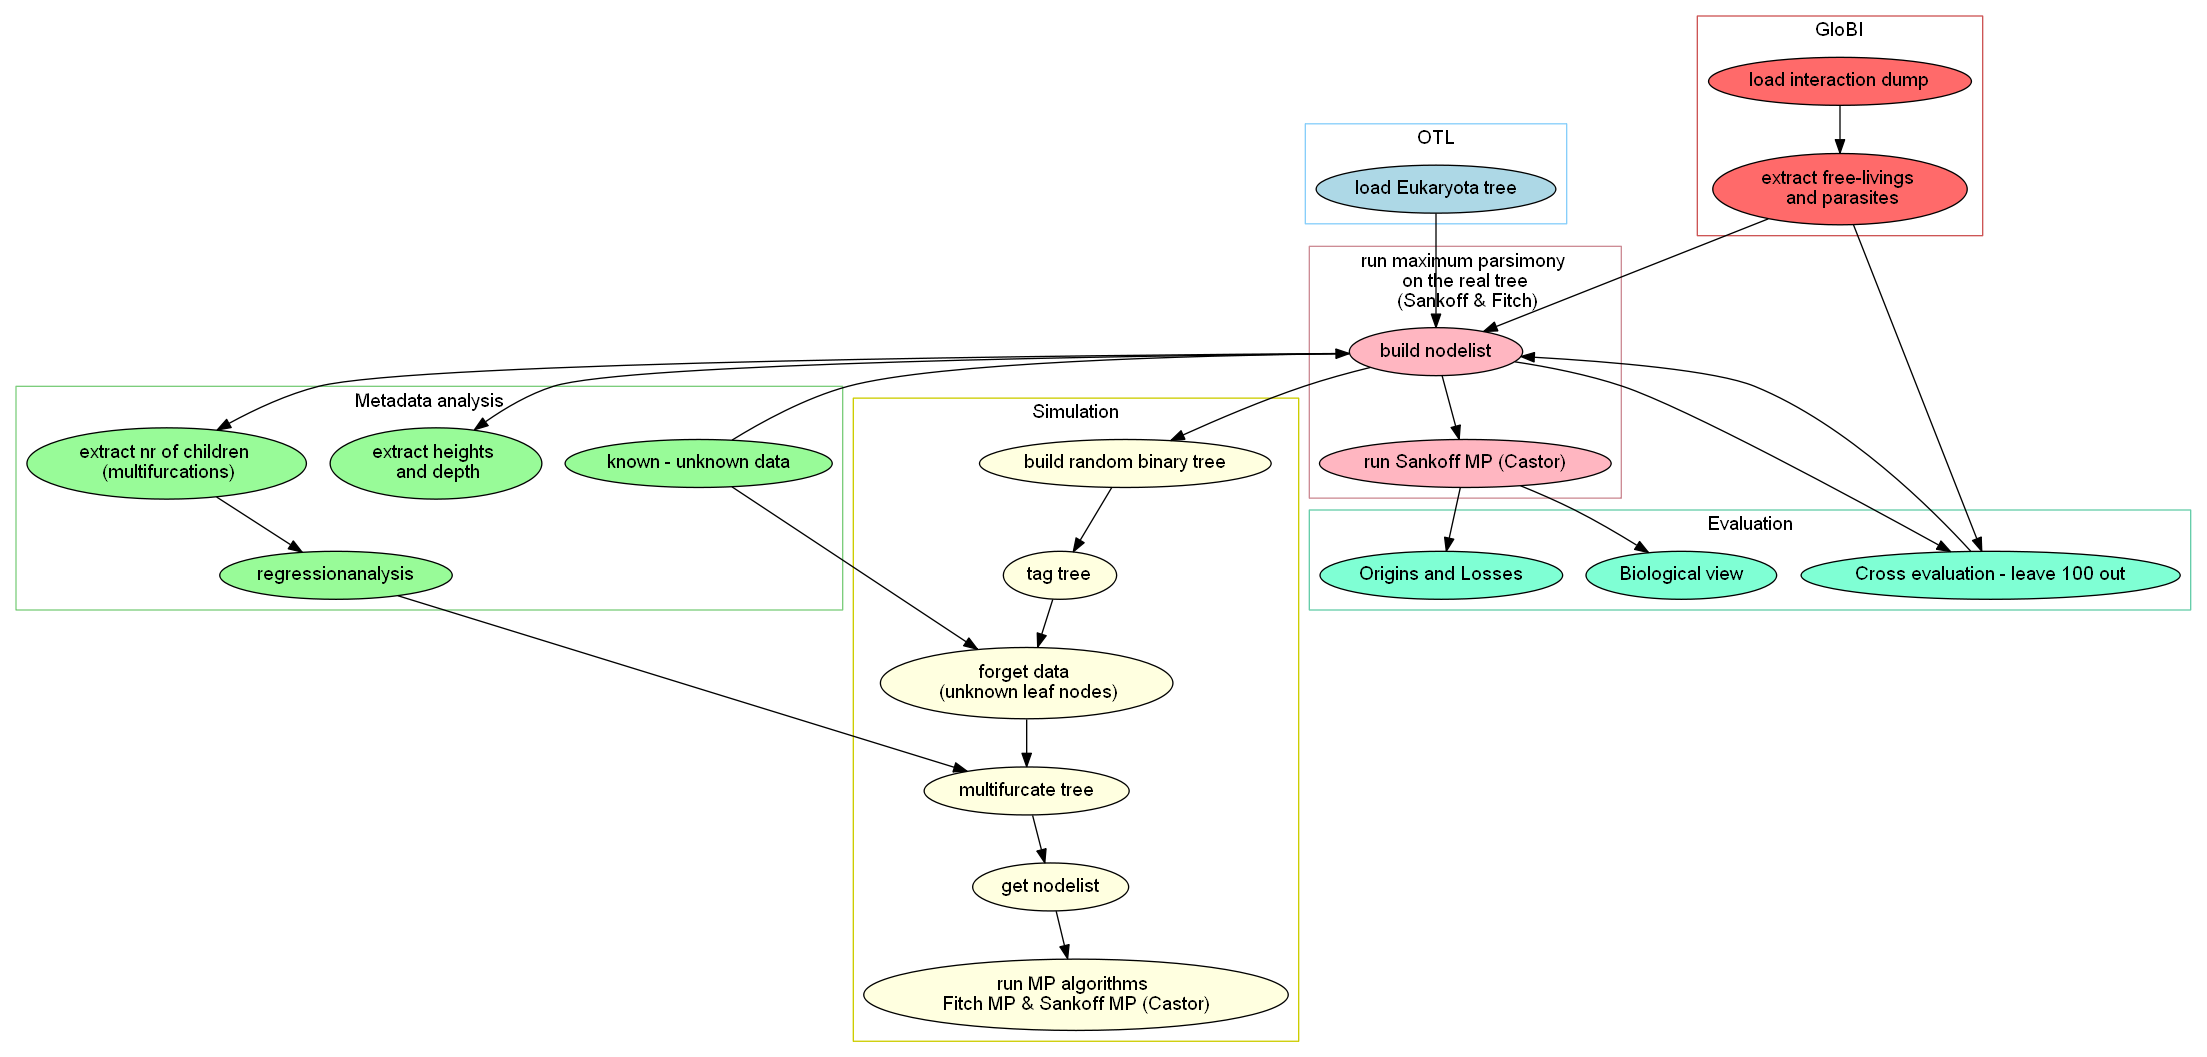
\includegraphics[angle=90, width=0.4\textwidth]{Figures/Workflow.png}
    %   \caption{Big overview of the whole Workflow}
    %   \label{fig:BigWorkflow}
    % \end{figure}
    \begin{figure}[h!]
      \centering
      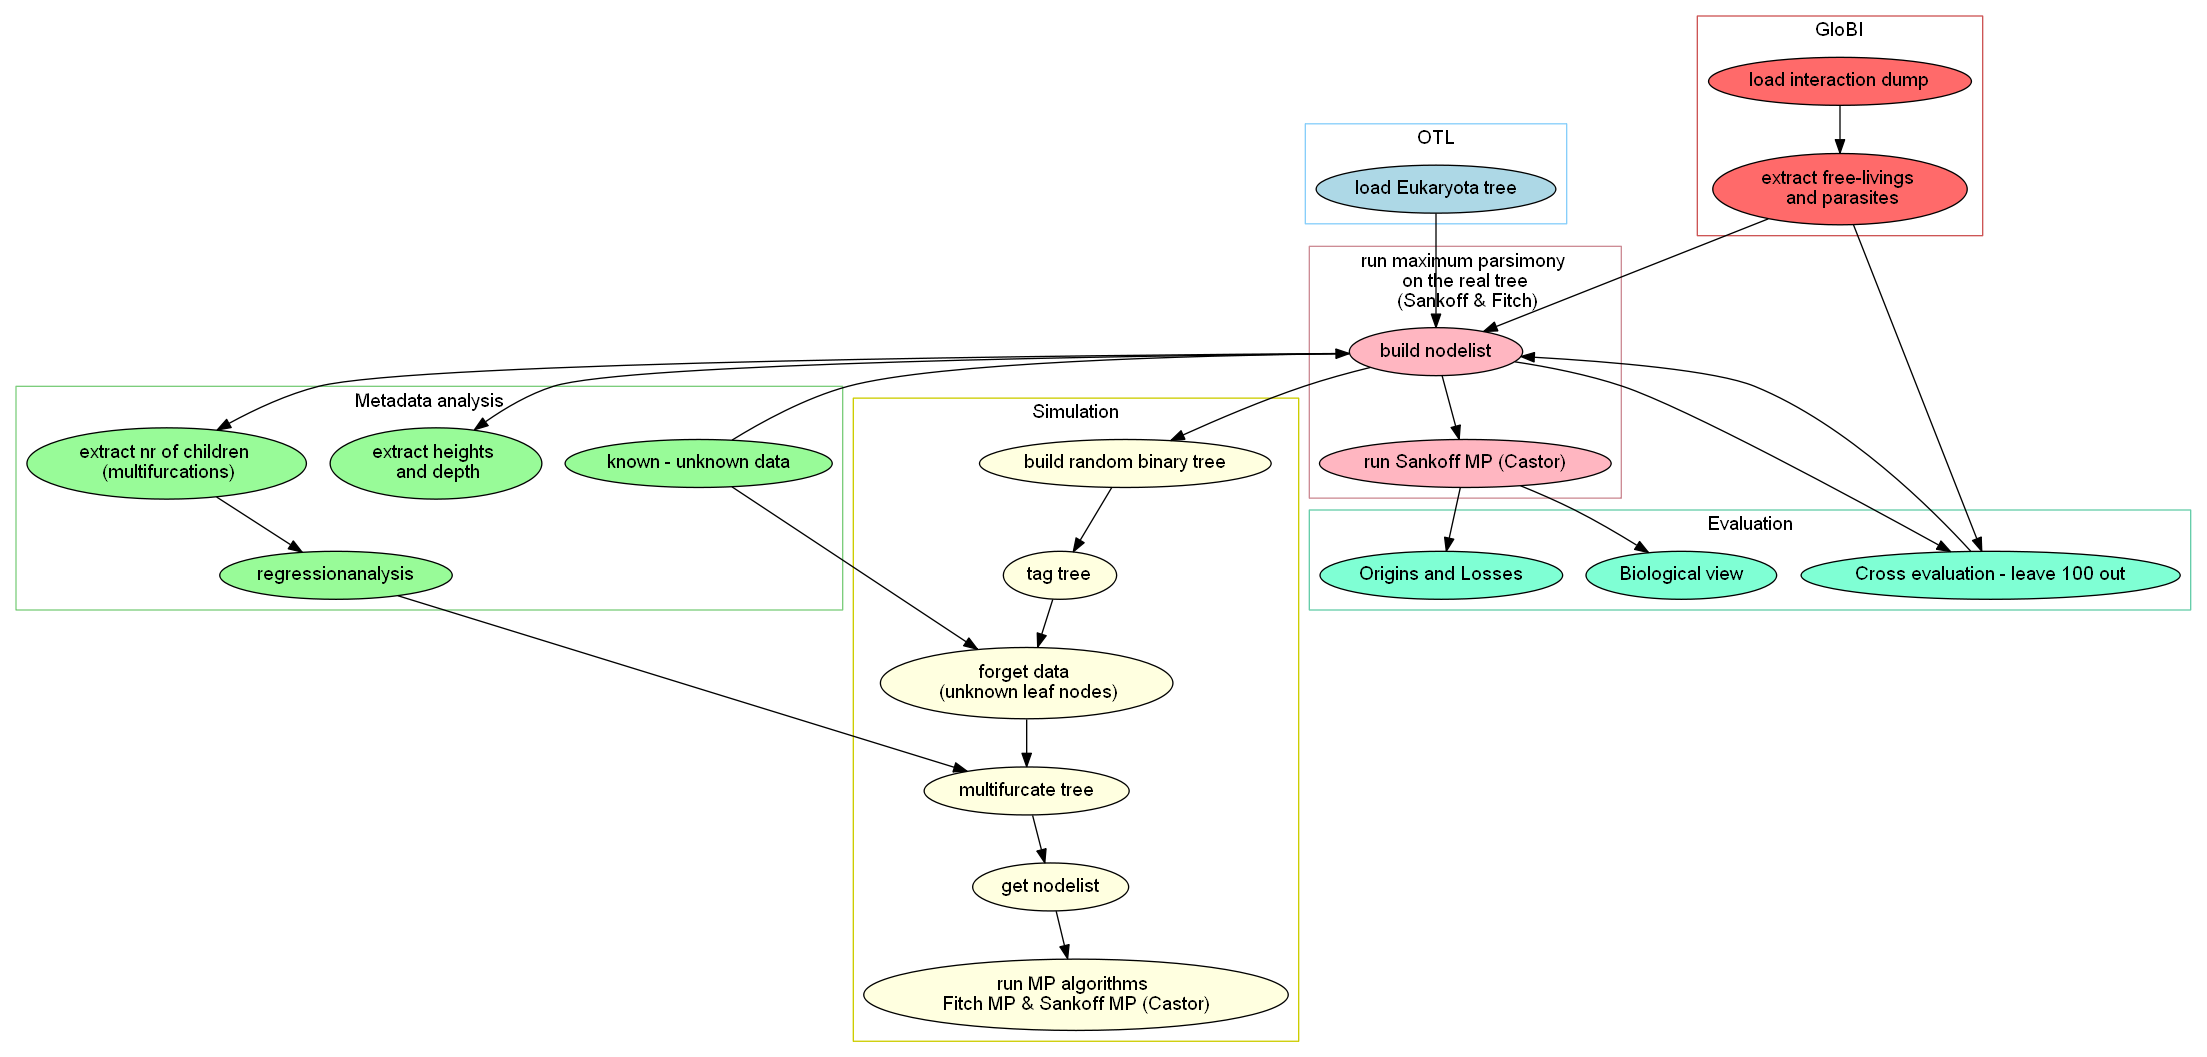
\includegraphics[width=\textwidth]{Figures/Workflow.png}
      \caption{Big overview of the whole Workflow}
      \label{fig:BigWorkflow}
    \end{figure}

  %---------------------------------------------------------------------------------------------------
  %---------------------------------------------------------------------------------------------------
  \section{OTL analysis}\label{sec:appendix - otl analysis}

    %---------------------------------------------------------------------------------------------------
    \subsection{List of all phyla}\label{subsec:listPhyla}

    Phyla (53): \\
    Acanthocephala, Amoebozoa, Apicomplexa, Arthropoda, Ascomycota, Bacillariophyta, Basidiomycota, 
      Brachiopoda, Bryozoa, Chaetognatha, Chlorophyta, Chordata, Chromerida, Chytridiomycota, 
      Ciliophora, Cnidaria, Colponemidia, Ctenophora, Cycliophora, Echinodermata, Entoprocta, 
      Entorrhizomycota, Euglenida, Foraminifera, Gastrotricha, Glomeromycota, Gnathostomulida, 
      Haplosporida, Haptophyta, Hemichordata, Kinorhyncha, Loricifera, Microsporidia, Mollusca, 
      Myzostomida, Nematoda, Nematomorpha, Nemertea, Onychophora, Orthonectida, Phaeophyceae, 
      Picozoa, Placozoa, Platyhelminthes, Porifera, Priapulida, Rhodophyta, Rhombozoa, Rotifera, 
      Streptophyta, Tardigrada, Xanthophyceae.

      Anthocerotophyta, Marchantiophyta, Bryophyta, Tracheophyta were found as phylum in the phylum 
        Streptophyta and Magnoliophyta as phylum in Tracheophyta and thus not included.

    %---------------------------------------------------------------------------------------------------
    \subsection{Distribution of Taxa}
      In the tree we can distinguish 28 different taxa in the OTL taxonomic tree. We sorted all taxa by
        rank into a table, counted their occurrences as internal nodes and leaf nodes (see table 
        \ref{table:taxa}) and plotted them as a diagram (see figure \ref{fig:taxa}).
    \begin{figure}[h!]
      \centering
      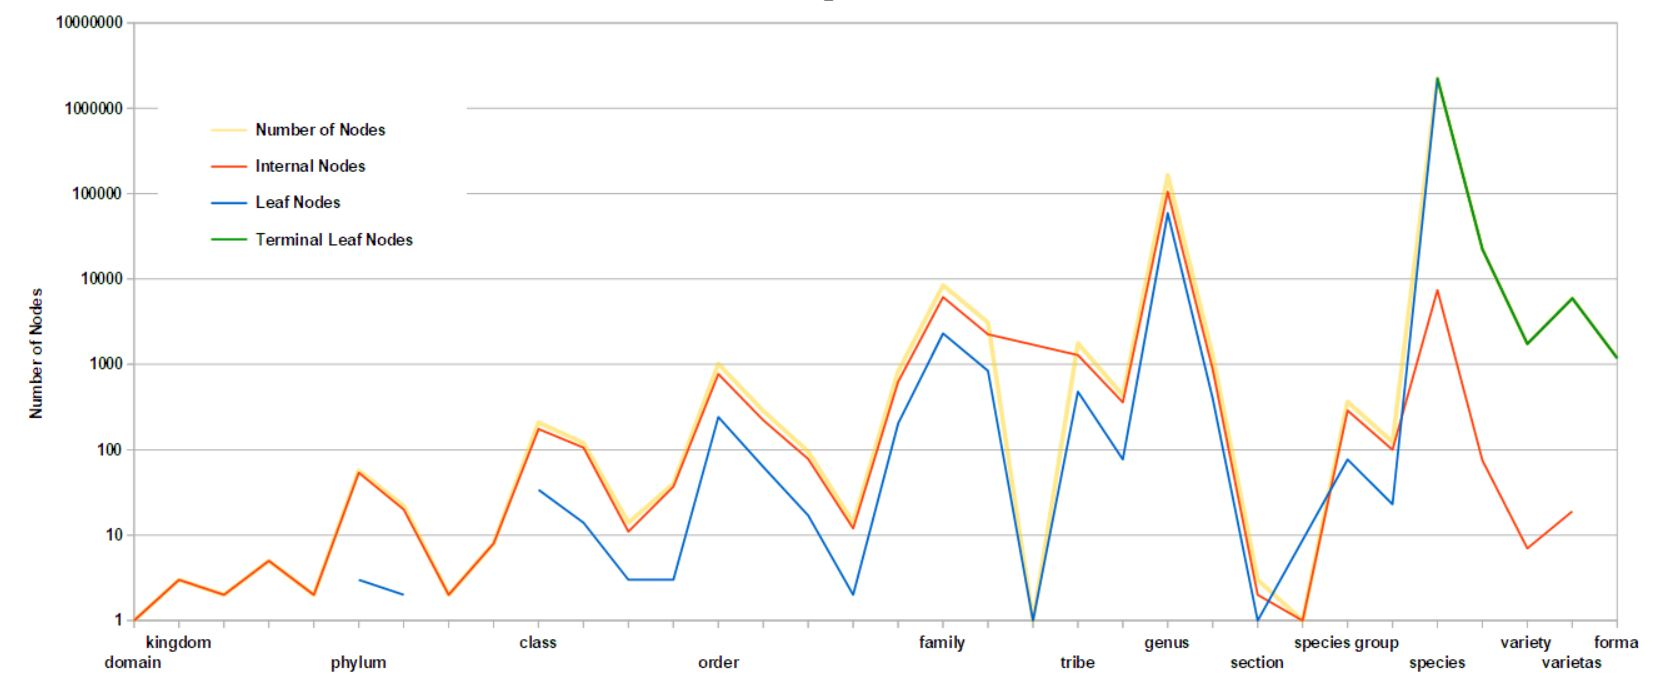
\includegraphics[width=\textwidth]{Figures/TaxaTable2.JPG}
      \caption{Distribution of Nodes in Rank-Cathegories}
      \label{fig:taxa}
    \end{figure}

    \begin{table}[h!]
      \begin{center}
        % \begin{tabular}{ |>{\rowmac}l|>{\rowmac}r|<{\clearrow} }
        \begin{tabular}{ |l|r||r|r| }
          \hline
          \bfseries Taxa & \bfseries Number of Nodes & \bfseries Internal Nodes & \bfseries Leaf Nodes \\
          \hline \hline
          \setrow{\bfseries}domain & 1        & 1 & - \\ \hline
          \setrow{\bfseries}kingdom & 3       & 3 & - \\
          subkingdom & 2                      & 2 & - \\
          infrakingdom & 5                    & 5 & - \\
          superphylum & 2                     & 2 & - \\ \hline
          \setrow{\bfseries}phylum & 57       & 57 & - \\
          subphylum & 22                      & 22 & - \\
          infraphylum & 2                     & 2 & - \\
          superclass & 8                      & 8 & - \\ \hline
          \setrow{\bfseries}class & 209       & 209 & - \\
          subclass & 120                      & 120 & - \\
          infraclass & 14                     & 14 & - \\
          superorder & 40                     & 40 & - \\ \hline
          \setrow{\bfseries}order & 1013      & 1013 & - \\
          suborder & 285                      & 285 & - \\
          infraorder & 95                     & 95 & - \\
          parvorder & 14                      & 14 & - \\
          superfamily & 829                   & 829 & - \\ \hline
          \setrow{\bfseries}family & 8442     & 8442 & - \\
          subfamily & 3090                    & 3090 & - \\
          supertribe & 1                      & 1 & - \\
          tribe & 1764                        & 1764 & - \\
          subtribe & 435                      & 435 & - \\ \hline
          \setrow{\bfseries}genus & 164592    & 164592 & - \\
          subgenus & 1266                     & 1266 & - \\
          section & 3                         & 3 & - \\
          subsection & 1                      & 1 & - \\
          species group & 308                 & 308 & - \\
          species subgroup & 108              & 108 & - \\ \hline
          \setrow{\bfseries}species & 2243241 & 18197 & 2225044 \\
          subspecies & 22378                  & 196 & 22182 \\
          variety & 1755                      & 29 & 1726 \\
          varietas & 5935                     & 61 & 5874 \\
          forma & 1179                        & & 1179 \\
          \hline \hline
          no rank & 951                       & 944 & 7 \\
          no rank - terminal & 37451          & - & 37451 \\
          (no entry) & 39816                  & 39816 & - \\
          \hline  
        \end{tabular}
        \caption{Distribution of Nodes in Rank-Cathegories}
        \label{table:taxa} 
      \end{center}  
    \end{table}

\newpage

  %---------------------------------------------------------------------------------------------------
  %---------------------------------------------------------------------------------------------------
  \section{Parasites in Chordata} \label{sec:parasites in chordata}
    We mapped the few parasitic species in a rough taxonomy (see Figure \ref{fig:ChordataParasites}): 
      Known parasitic birds belong to the order Sauria. Here we know from Rothschild that there are 
      breeding parasites like the cuckoo and clepto-parasites like the skua  \cite{Rothschild1957}. We
      received 6 input parasites from GloBI and got no predictions: A woodpecker - 
      \textit{Sphyrapicus varius} and a duck - \textit{Aix sponsa}, a cow bird - \textit{Molothrus ate} 
      known as broodparasite and some others.
      
    An example of the amplification of mistakes are the carp. There is a paper from which GloBI 
      concludes: the Grass carp (\textit{Ctenopharyngodon idella)} has as pathogen the common carp 
      (\textit{Cyprinus carpio})\footnote{
        \hyperlink{https://www.globalbioticinteractions.org/?interactionType=hasParasite&targetTaxon=Cyprinus\%20carpio}
        {https://www.globalbioticinteractions.org/?interactionType=hasParasite\&targetTaxon=Cyprinus\%20carpio};
        Last checked: 22.03.2018.
      }. Since there is hardly any information about free-living, it follows that all siblings are 
      also predicted to be parasitic.

    \begin{figure}[h!]
      \centering
      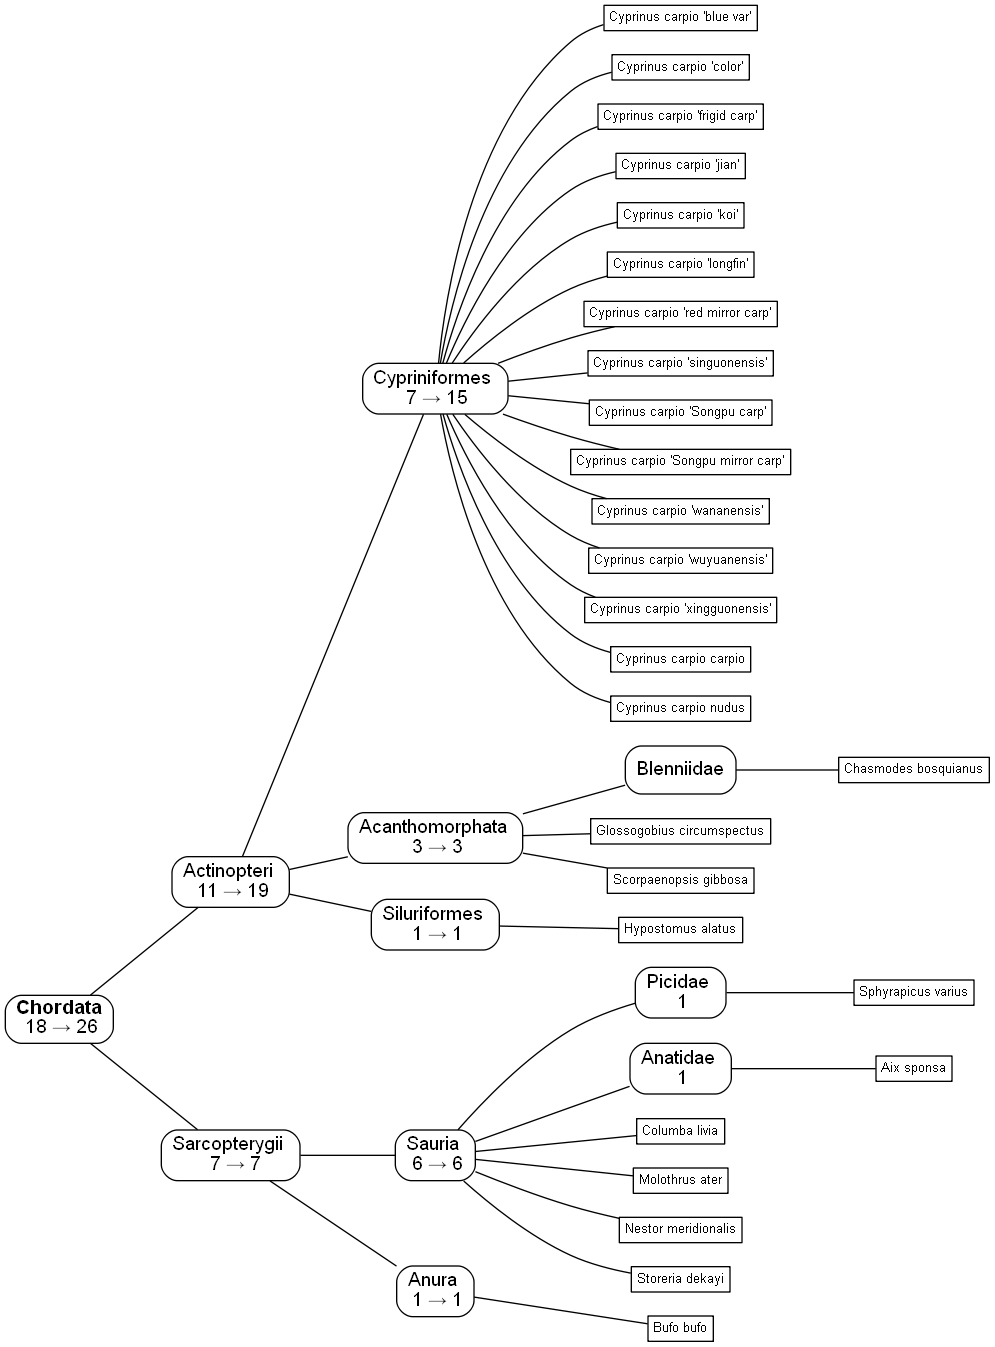
\includegraphics[trim = 0mm 0mm 0mm 0mm, clip, width=0.85\textwidth]{Figures/ChordataParasites.png}
      \caption{Parasites of Phylum: Chordata. \\
        All parasite data of the Chordata is mapped into a rough taxonomy (phylum, class, order, 
          family) in order to understand its distribution and affiliation. \\
        The internal nodes are the wanted taxa from OTL (with the addition of \# input parasites to 
          $\rightarrow$ \# predicted parasites). \\
        The leaf nodes are the input parasites (green) and the predicted parasites (white $\rightarrow$ 
          green).}
      \label{fig:ChordataParasites}
    \end{figure}

\end{document}